% Create a Table of Contents in Beamer
\documentclass[10pt,t]{beamer}
% Theme choice:
\usetheme{Singapore}
\usecolortheme{whale}
\setbeamercolor{titlelike}{fg=blue,bg=white}
\setbeamercolor{frametitle}{fg=blue,bg=white}
\setbeamertemplate{frametitle}[default][left]
\setbeamertemplate{navigation symbols}{}

\usepackage{graphicx}
\usepackage{amsmath}
\usepackage{amsfonts}
\usepackage{amssymb}
\usepackage{amsthm}
\usepackage{ulem}

% Title page details: 
\title{Chapter 1: Linear Regression} 
\author{Taylor Okonek \& Charlie Wolock}
\date{\today}


\begin{document}
	% Title page frame
	\begin{frame}
	\titlepage 
\end{frame}

\begin{frame}{Learning objectives}
By the end of Chapter 1, you should be able to:
\begin{itemize}
	\item Formulate a regression model, given a scientific or statistical question
	\item Interpret the coefficients for a (simple or multiple) linear regression model
	\item Interpret confidence intervals and p-values for linear regression coefficients
	\item Classify variables according to their role in a linear regression model (e.g., outcome, predictor, potential confounder, effect modifier, precision variable)
	\item Use \texttt{R} to fit a linear regression model (and know where in the output to look for the information we need to interpret results)
	\item Create graphs to support your linear regression analysis
\end{itemize}
\end{frame}

% Outline frame
\begin{frame}{Outline}
\tableofcontents
\end{frame}

\AtBeginSection[ ]
{
\begin{frame}{Outline}
\tableofcontents[currentsection]
\end{frame}
}

% Presentation structure
\section{Simple Linear Regression}

\begin{frame}{Simple linear regression}

We collect 150 leaves, and record their lengths and widths in inches. We hypothesize that leaves with larger lengths will also tend to have larger widths. To represent this graphically, we plot all of the data below\dots

\vspace{0.3cm}

\begin{figure}
	\centering 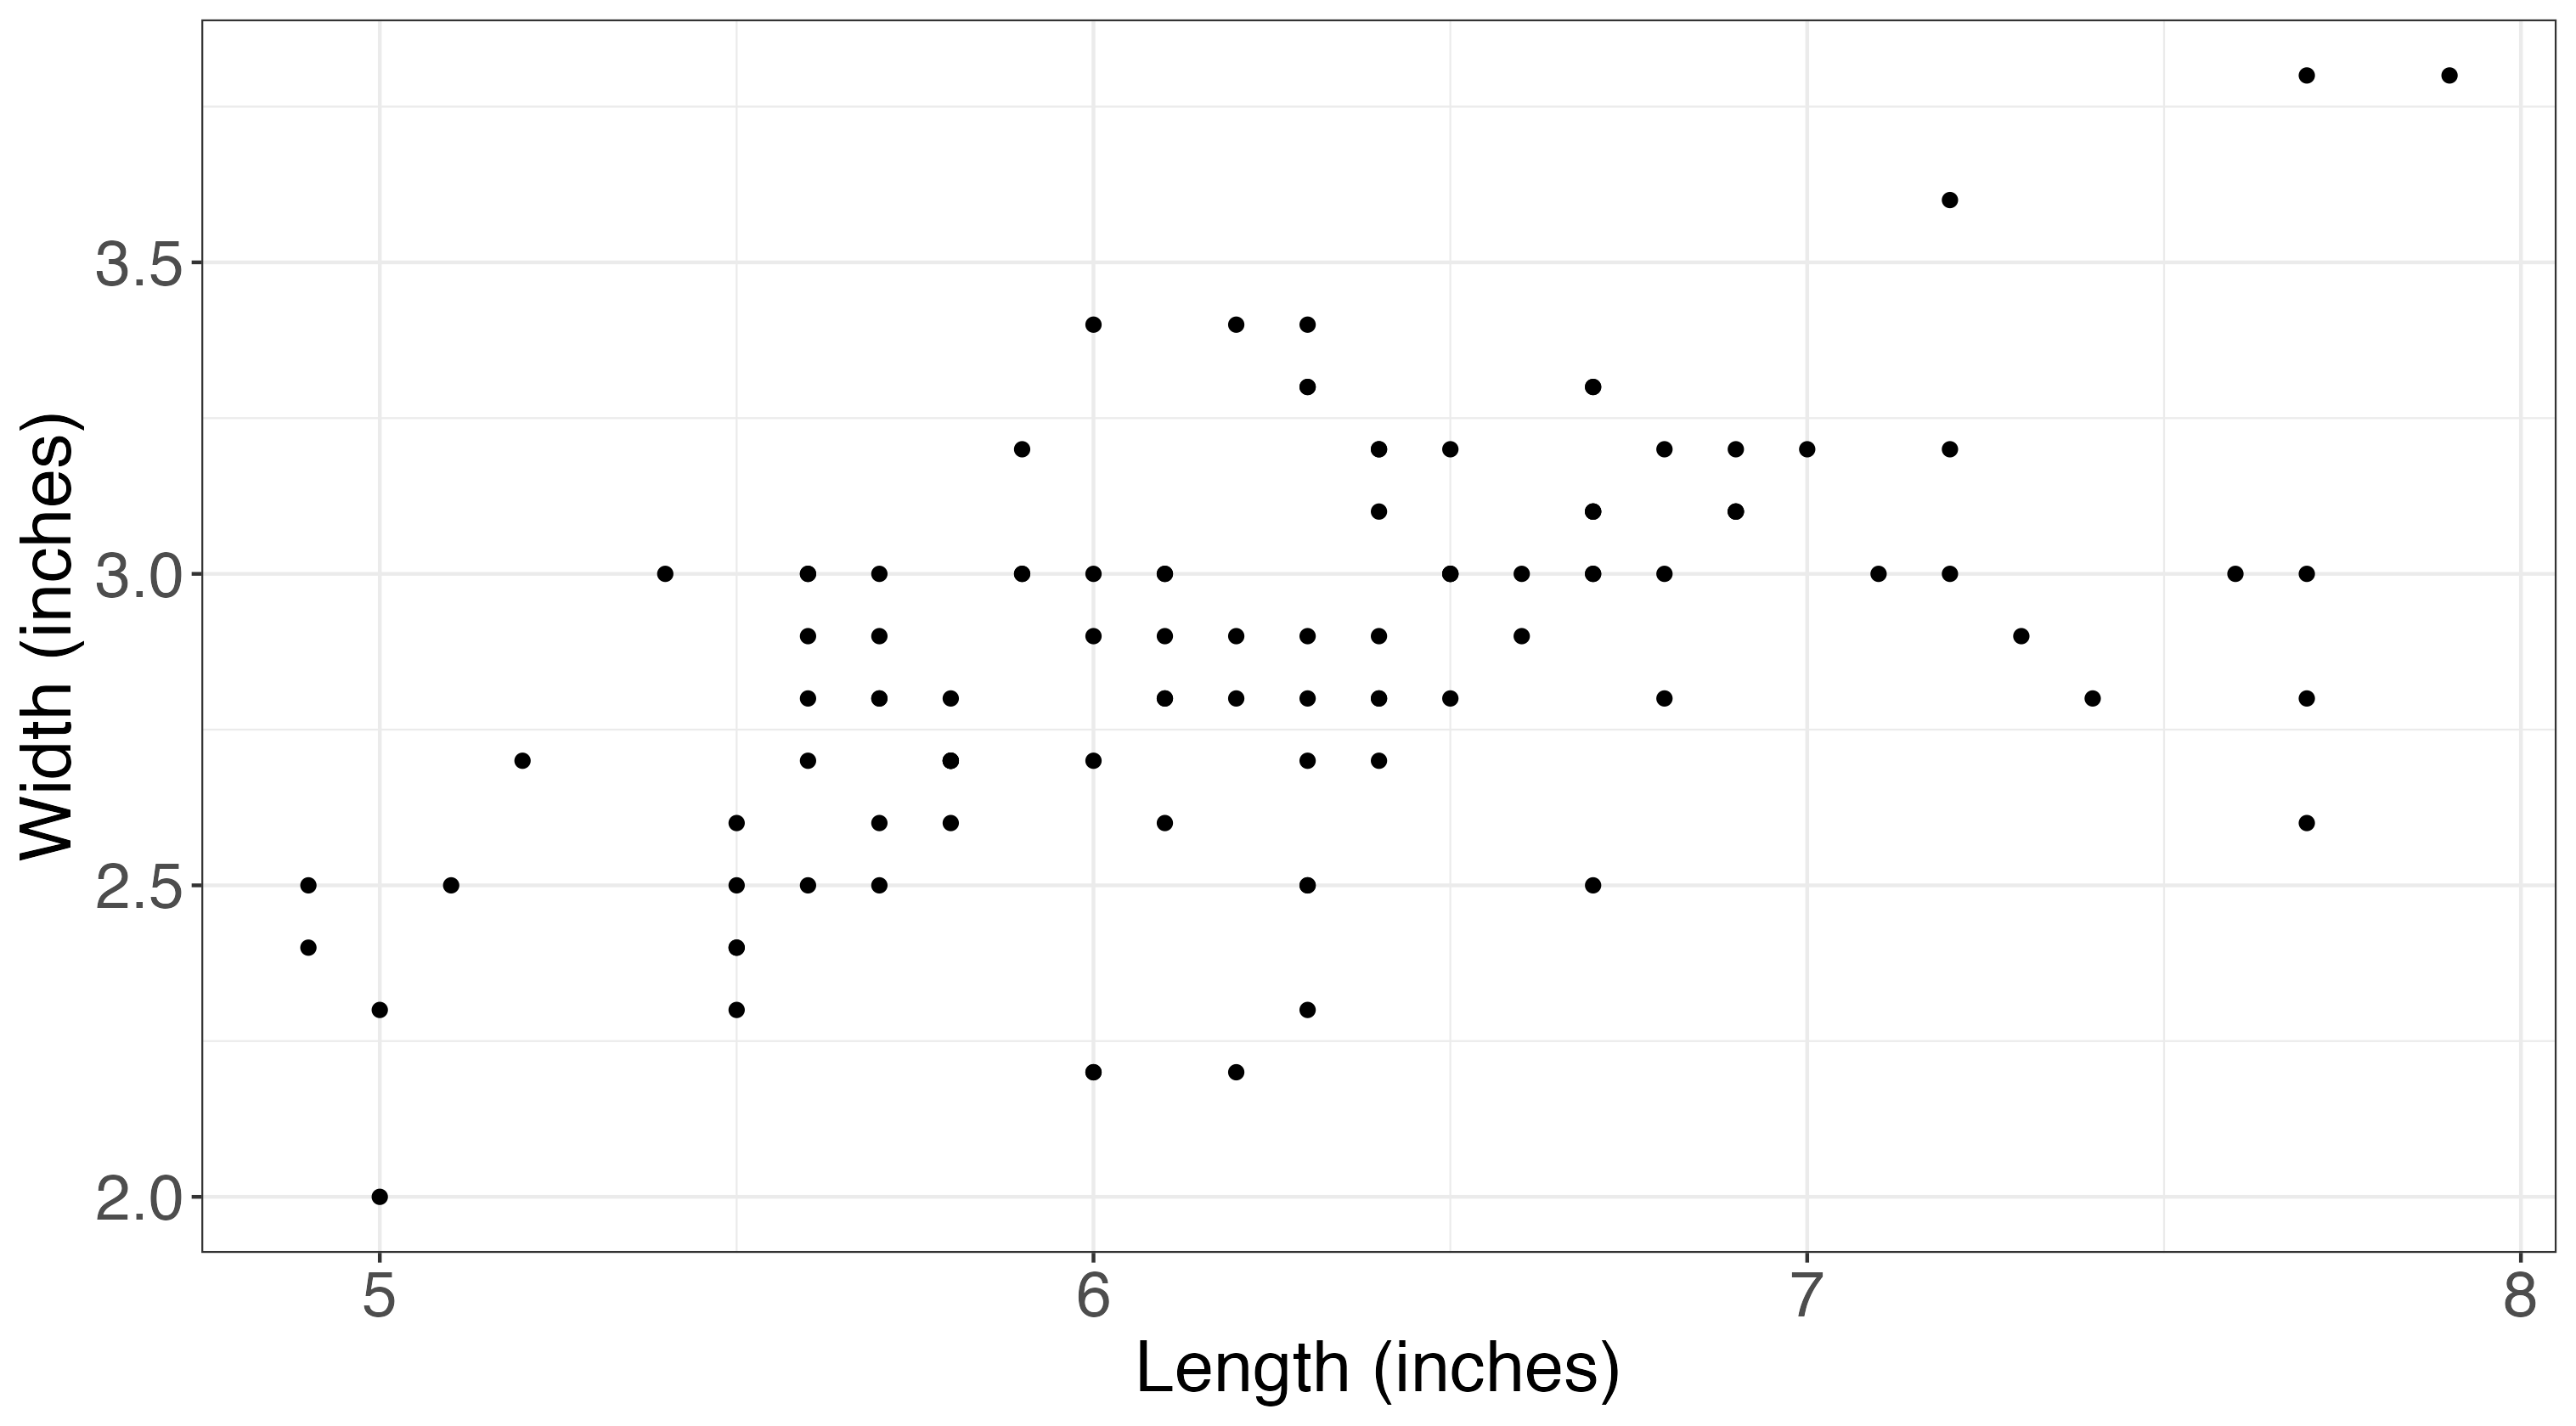
\includegraphics[scale=0.35]{points.png}
\end{figure}

\end{frame}

\begin{frame}{Simple linear regression}
Suppose we want to know how length and width are \textit{linearly} related to each other. To do this, we need to draw a line (\textcolor{red}{$y = a + bx$}) through our data:

\vspace{0.3cm}
\begin{figure}
\centering 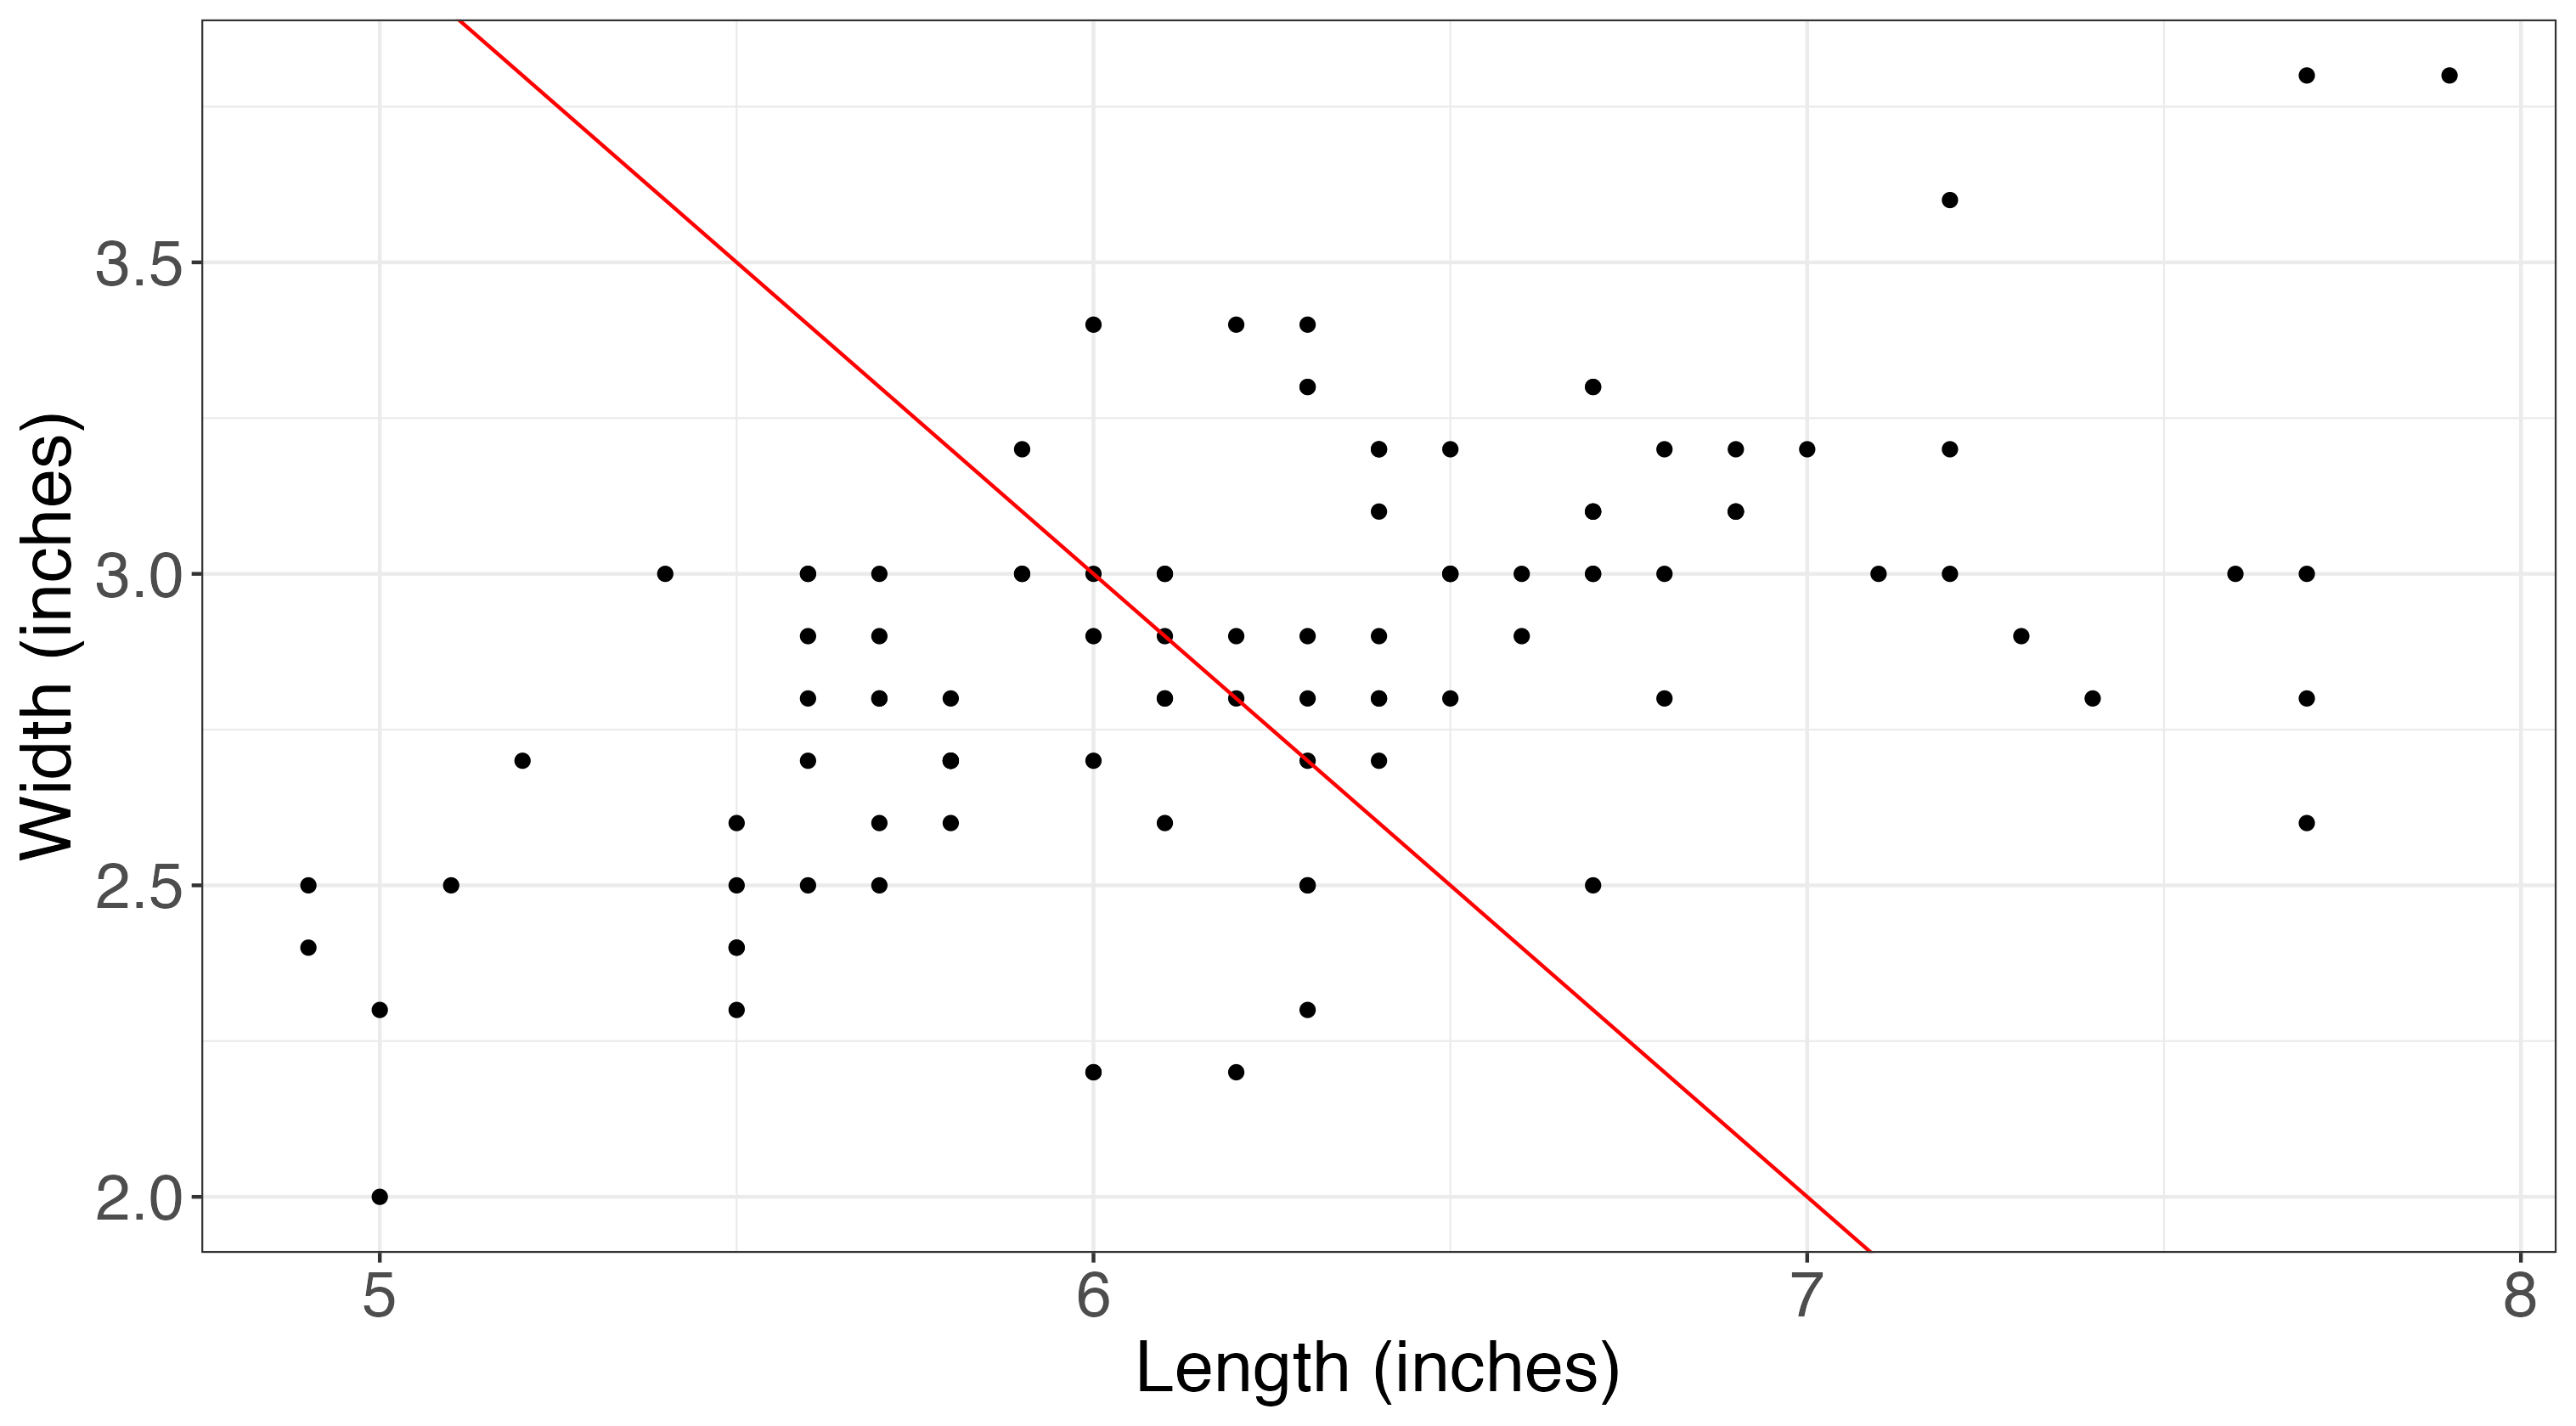
\includegraphics[scale=0.35]{points2.png}
\end{figure}

\end{frame}

\begin{frame}{Simple linear regression}


\begin{figure}
	\centering 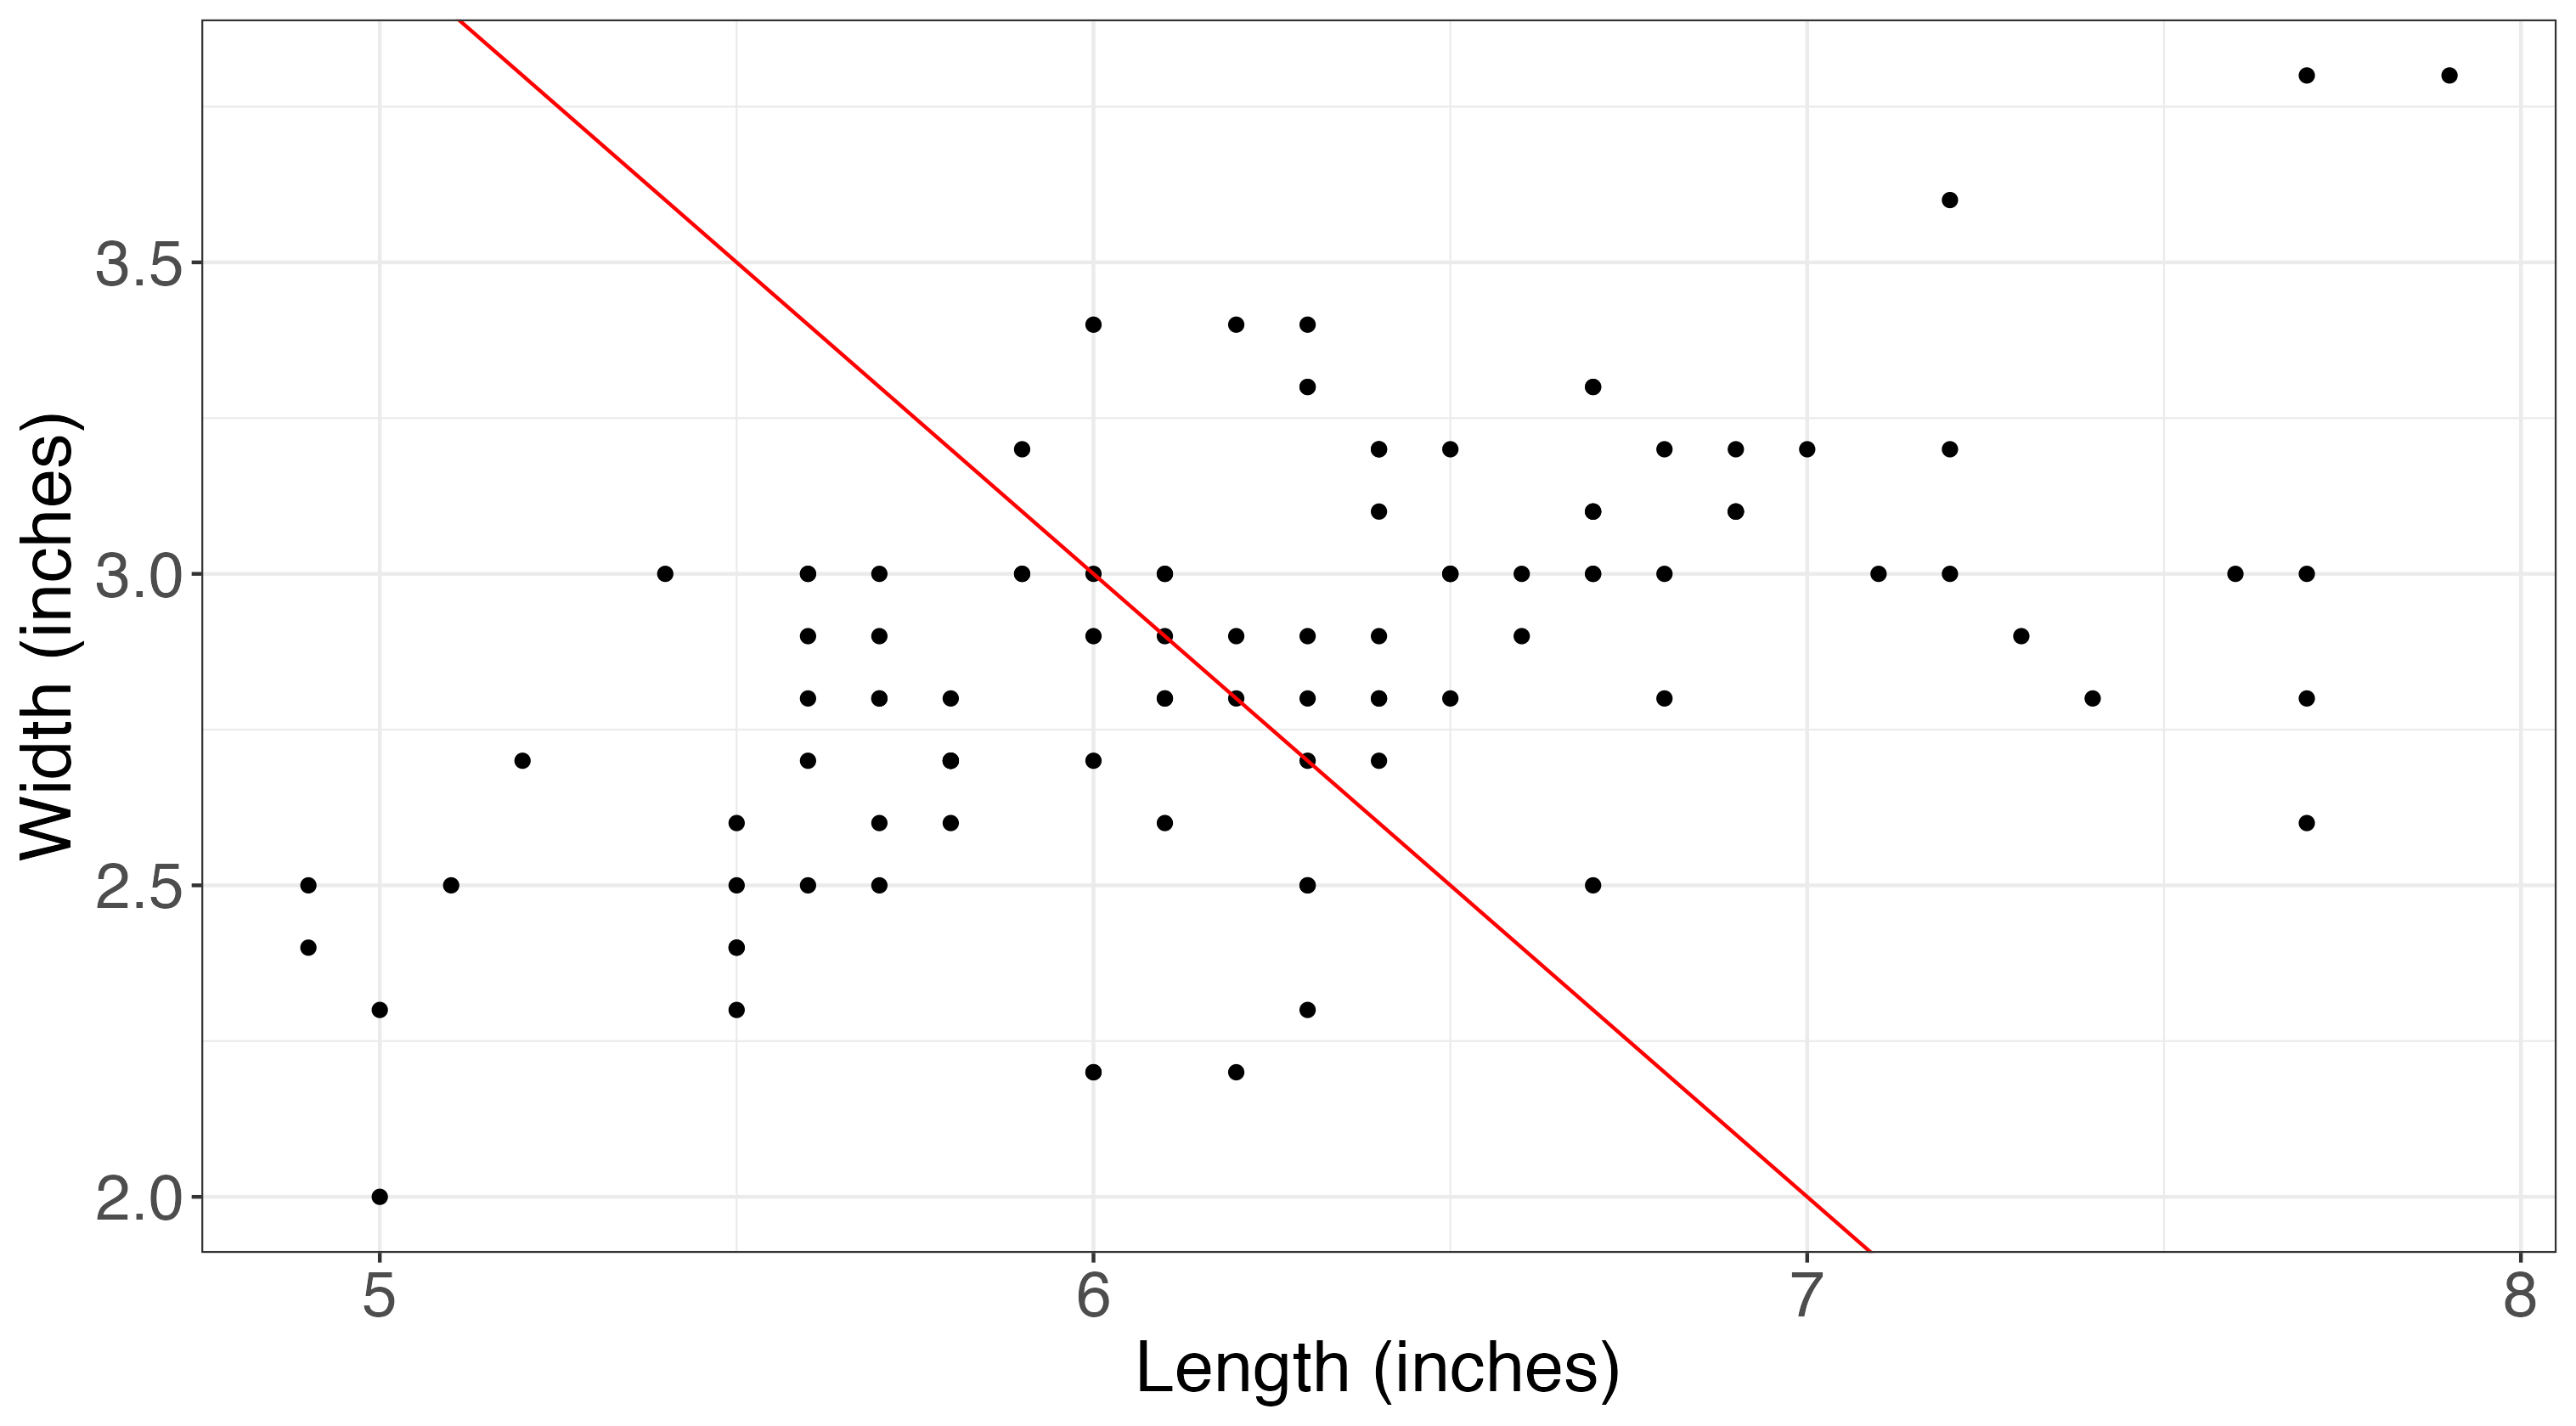
\includegraphics[scale=0.35]{points2.png}
\end{figure}

\vspace{0.3cm}

This line seems bad. Can we articulate \textit{why} it seems bad? Can we articulate why it seems bad \textit{mathematically}?

\end{frame}

\begin{frame}{Simple linear regression}

\begin{figure}
	\centering 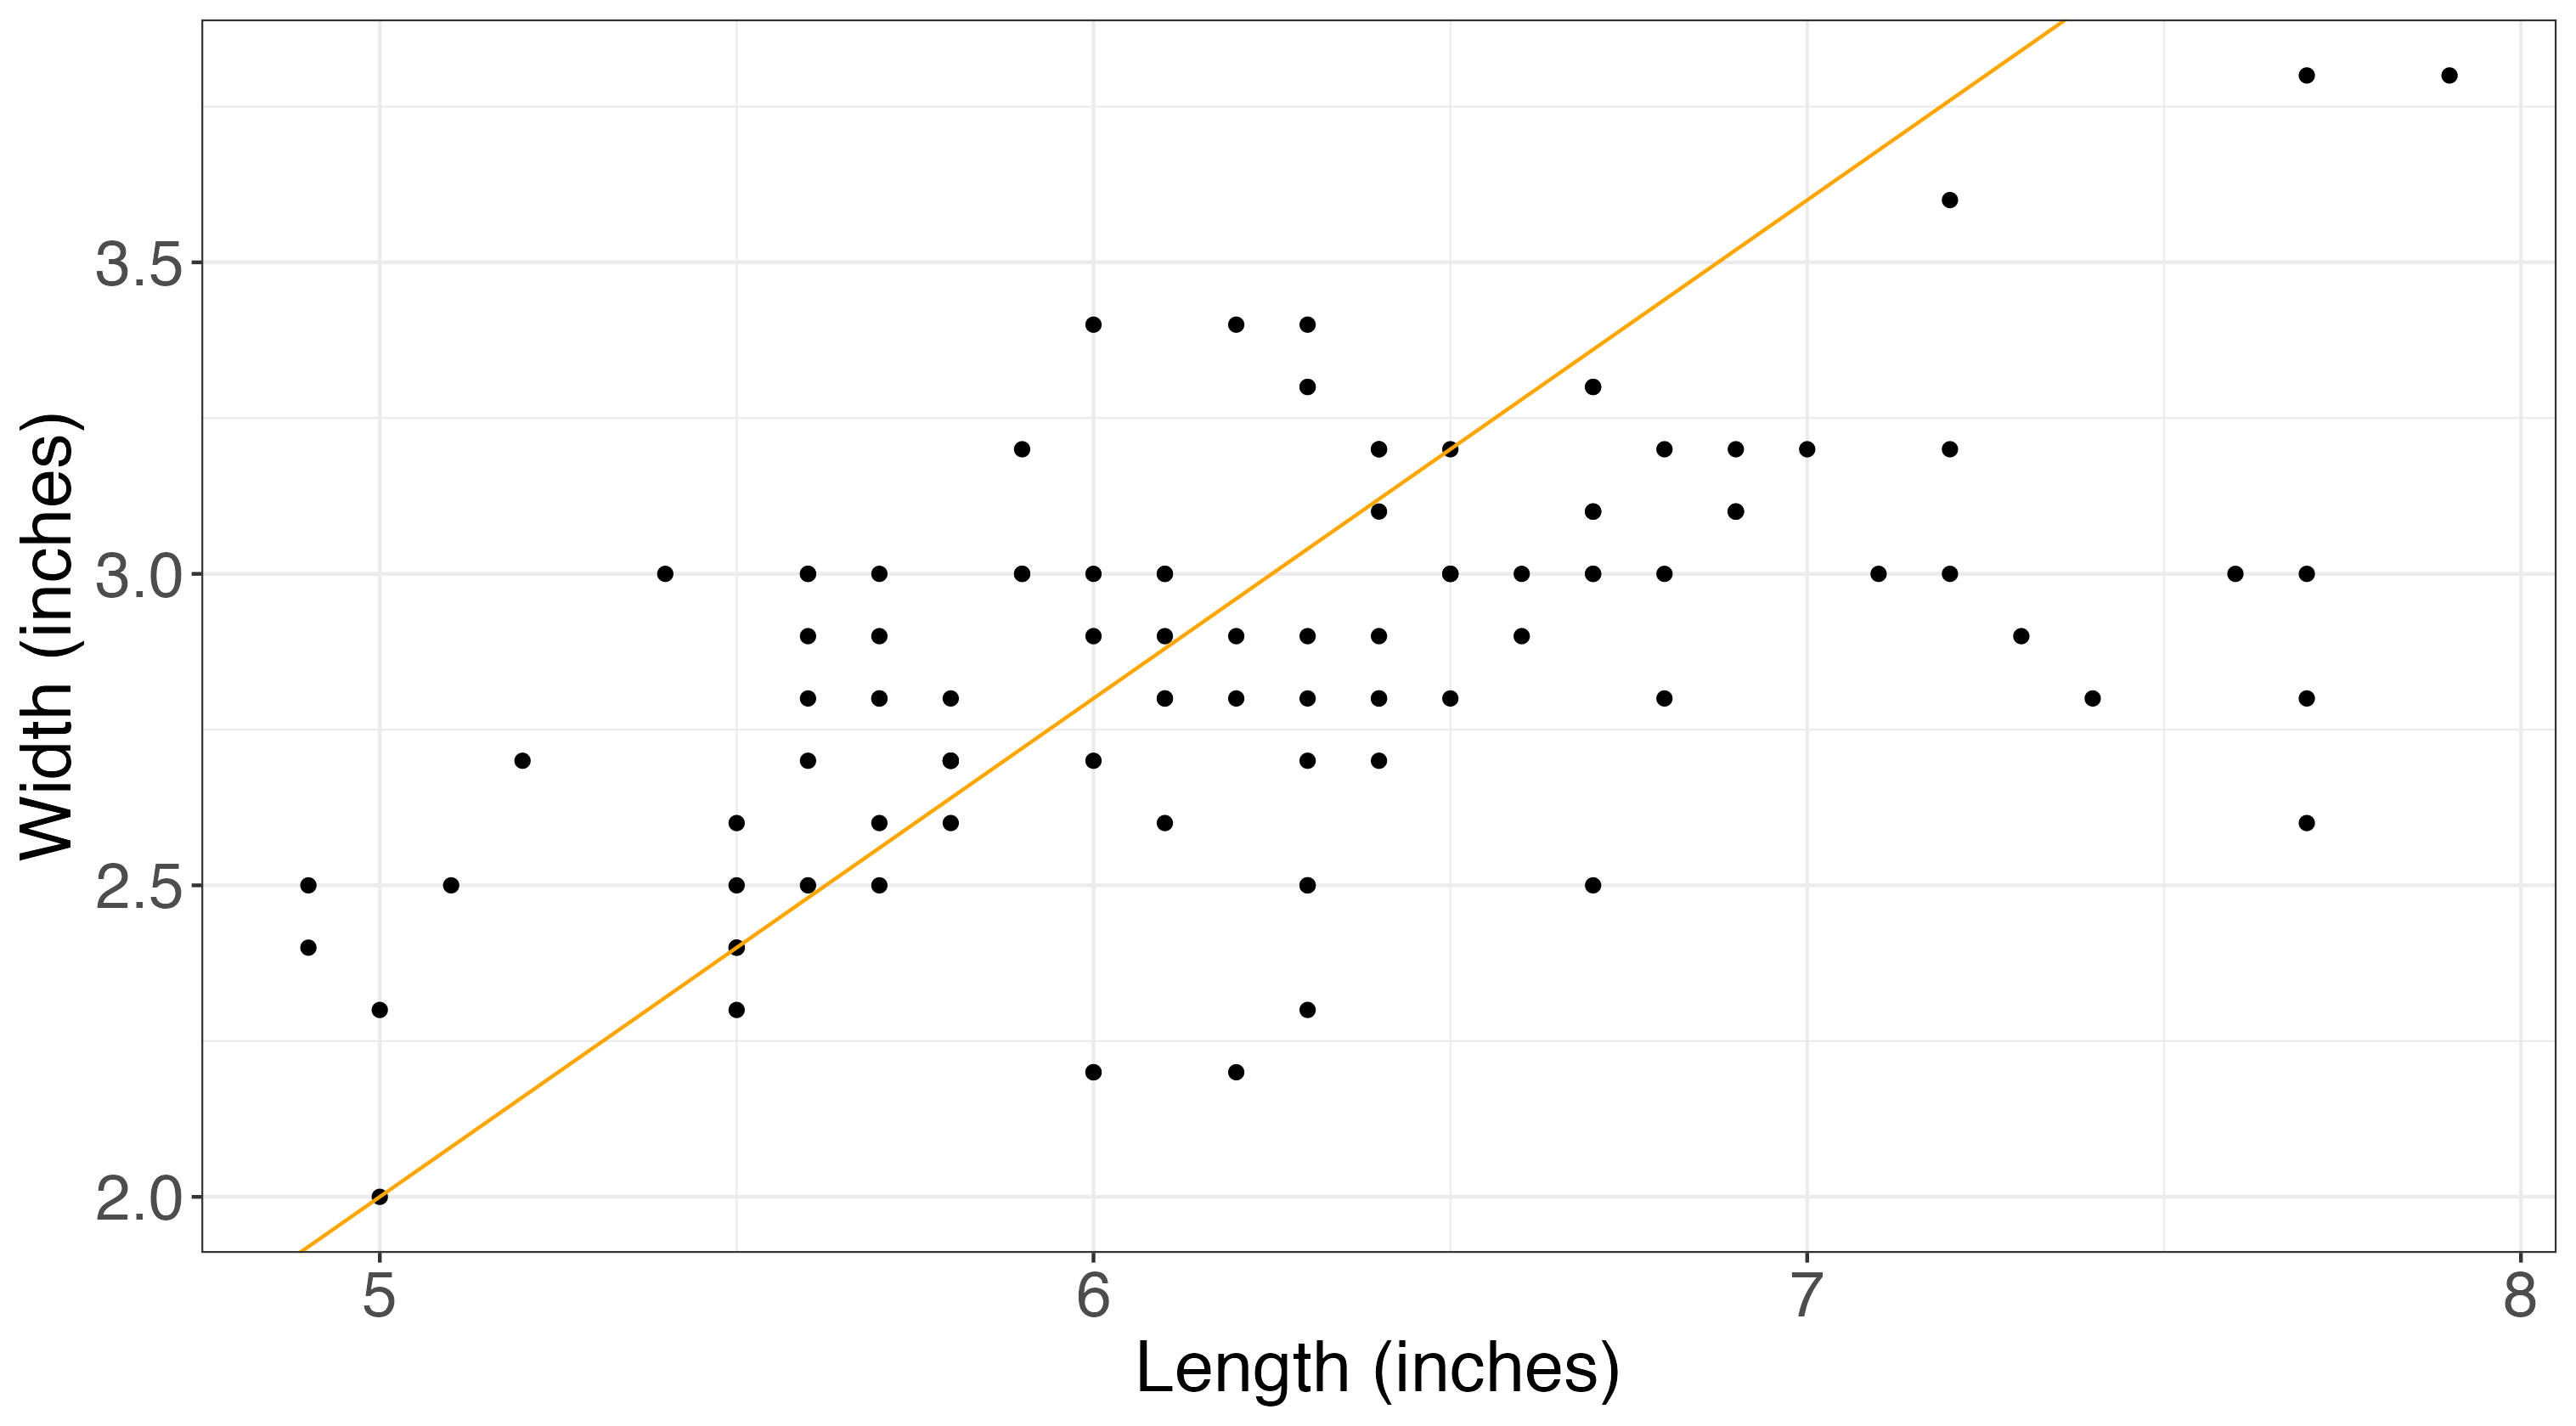
\includegraphics[scale=0.35]{points3.png}
\end{figure}

\vspace{0.3cm}
\small This line seems better! But is it the \textit{best}? And how do we define best?

\end{frame}

\begin{frame}{Simple linear regression}
Simple linear regression is a statistical tool that allows us to estimate the ``best" fitting line through two variables. In general, we use linear regression with \textbf{quantitative} outcomes. Below we show our guesses for the best fitting line and the line estimated from simple linear regression in \textcolor{blue}{blue}:

\begin{figure}
	\centering 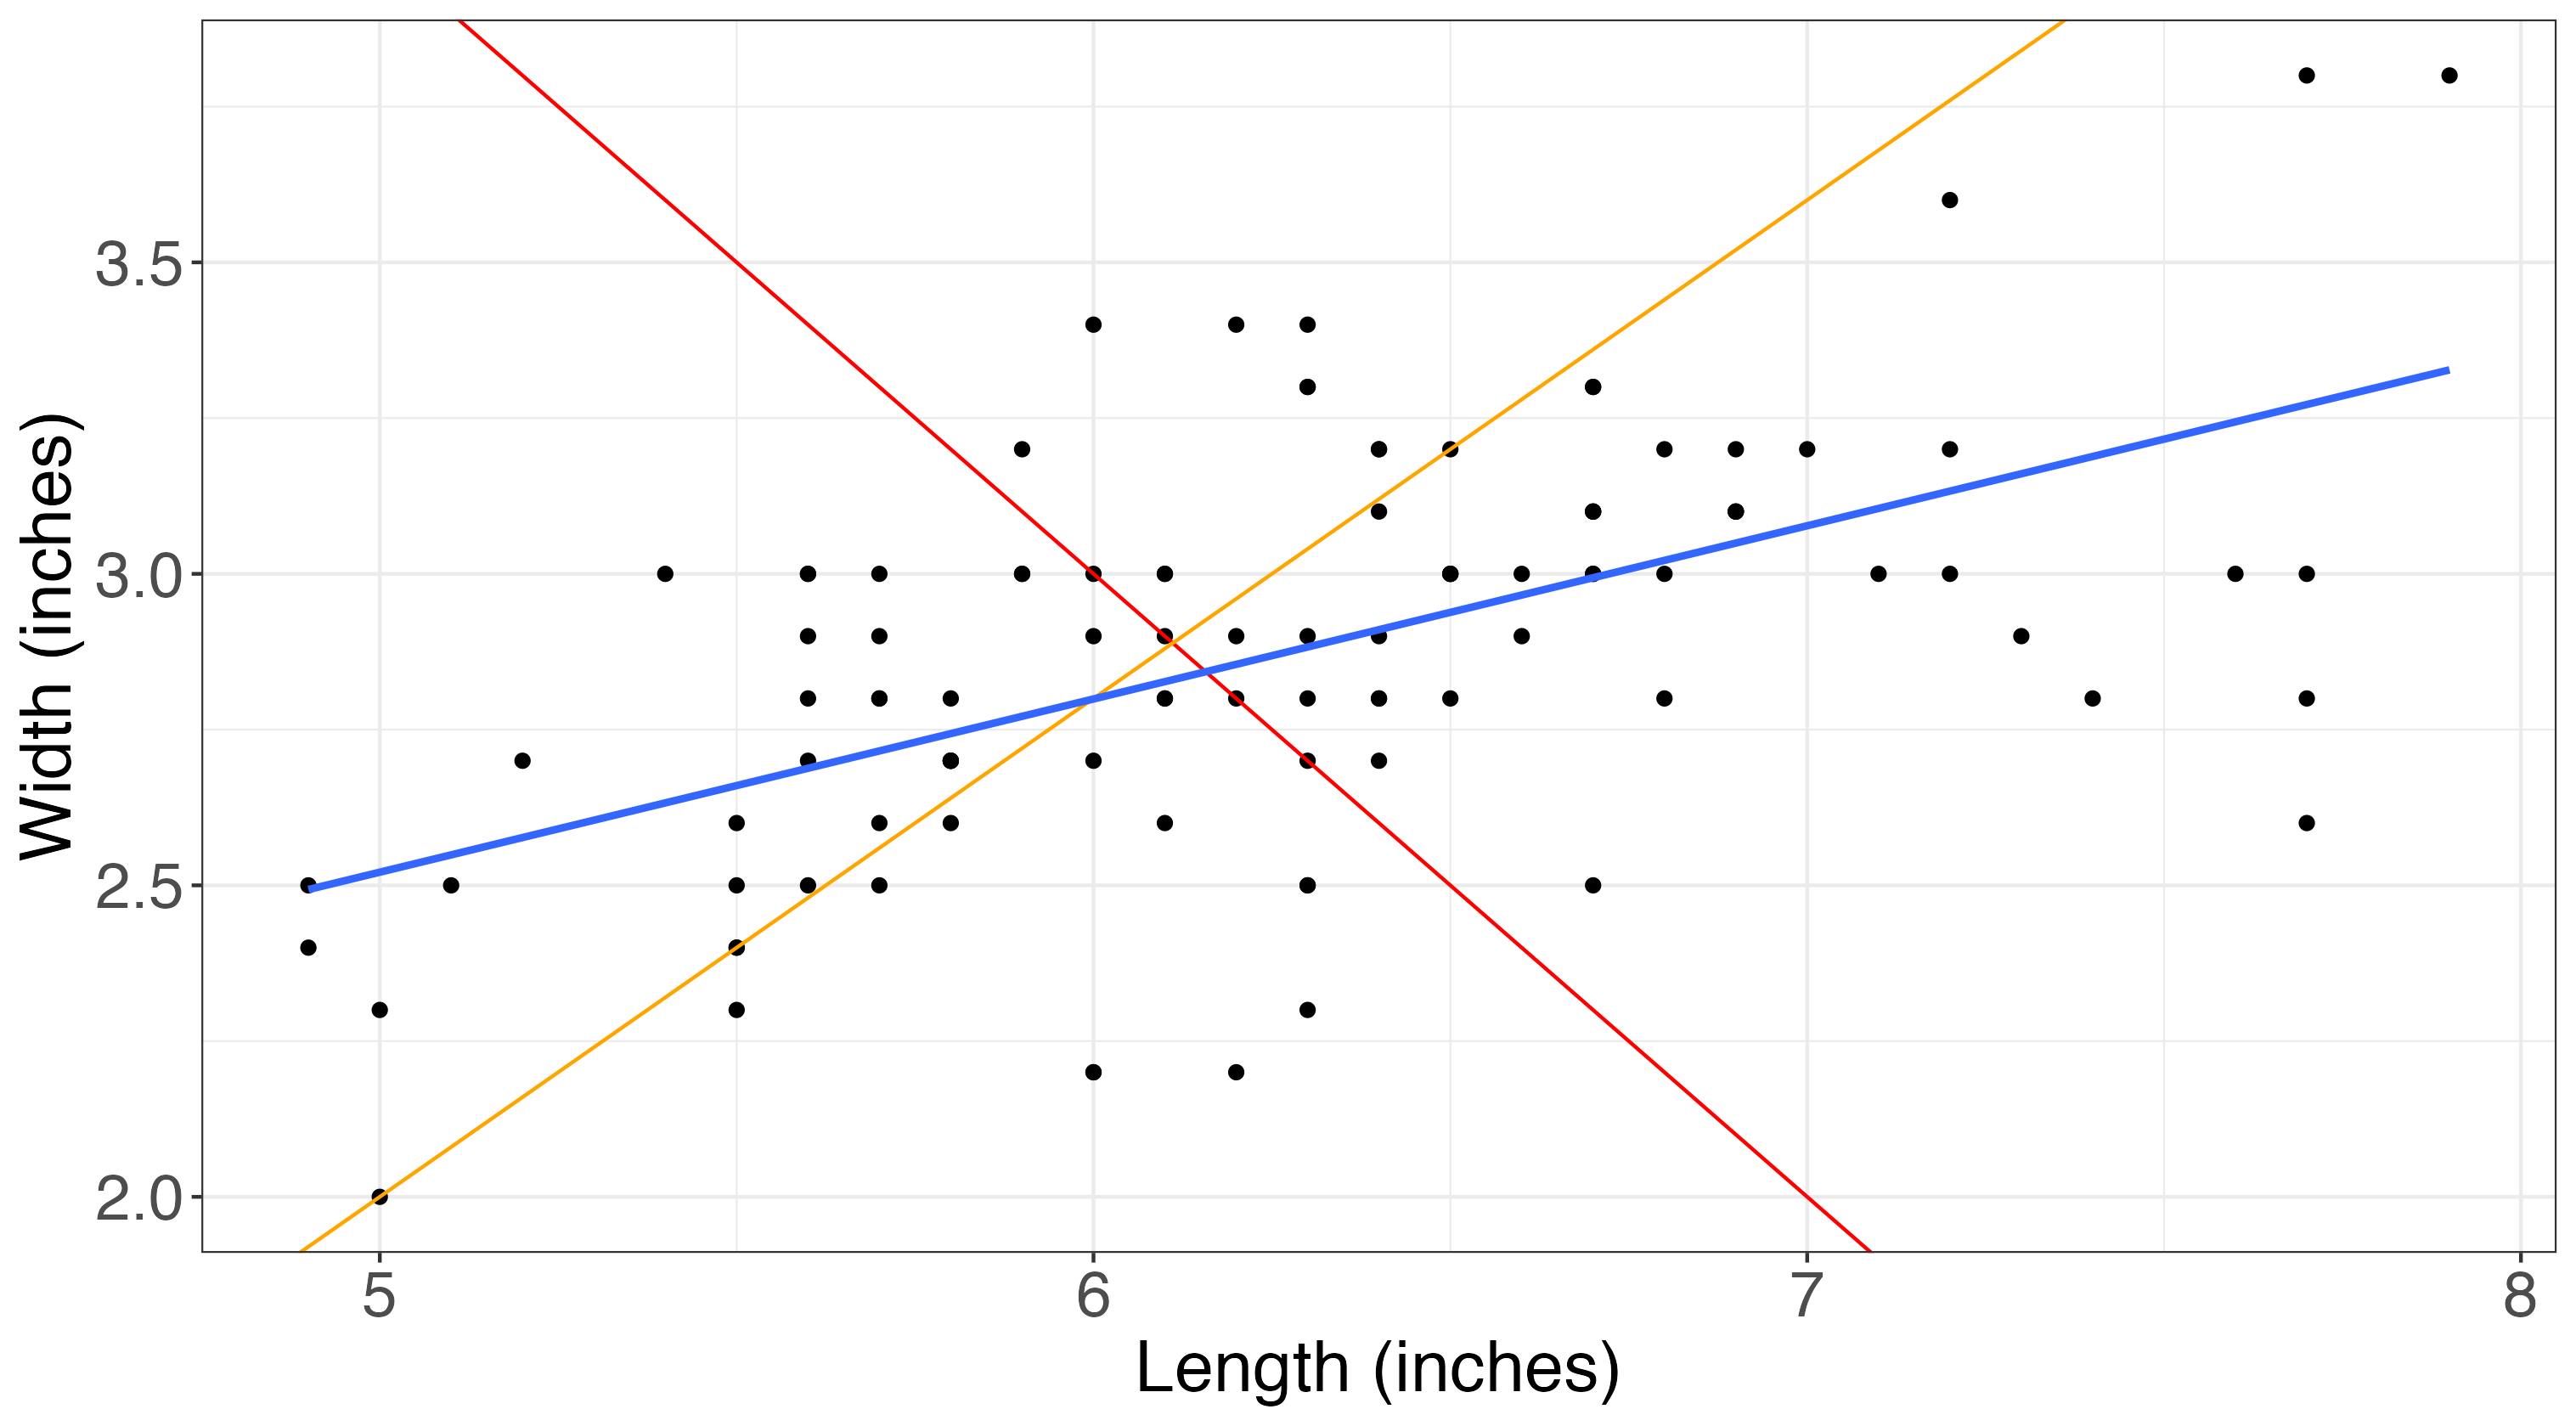
\includegraphics[scale=0.35]{points4.png}
\end{figure}

\end{frame}

\begin{frame}{Simple linear regression}
Lines take the form \textcolor{red}{$y = a + bx$}. When writing regression models we'll use the notation $E[Y \mid X] = \beta_0 + \beta_1 X$. Translating this, we have

\vspace{0.3cm}

\begin{itemize}
	\item $\beta_0$: The intercept of the linear regression line
	\item $\beta_1$: The slope of the linear regression line
	\item $E[Y]$: The average value of $Y$ in the population
	\item $E[Y \mid X]$: The average value of $Y$ in the population, given the predictor $X$
\end{itemize}
\end{frame}

\begin{frame}{Simple linear regression}
Lines take the form \textcolor{red}{$y = a + bx$}. When writing regression models we'll use the notation $E[Y \mid X] = \beta_0 + \beta_1 X$. Translating this, we have

\vspace{0.3cm}

\begin{itemize}
	\item $\beta_0$: The intercept of the linear regression line
	\item $\beta_1$: The slope of the linear regression line
	\item $E[Y]$: The average value of $Y$ in the population
	\item $E[Y \mid X]$: The average value of $Y$ in the population, given the predictor $X$
	\item Examples: $Y$ is birthweight, $X$ is participation in First Steps
	\begin{itemize}
		\item $E[Y] = 3414$ grams (average birthweight in the population)
		\item $E[Y \mid X = 0] = 3424.7$ grams (average birthweight for those not in FS)
		\item $E[Y \mid X = 1] = 3358.5$ grams (average birthweight for those in FS)
	\end{itemize}
\end{itemize}
\end{frame}

\begin{frame}{Simple linear regression: types of predictors}
Our example with heights and widths of leaves had a quantitative outcome \textit{and} a quantitative predictor. 

\vspace{0.3cm}

We can also do simple linear regression with other types of predictors, such as binary or categorical (the illustrative plots just don't look quite as nice). In HW2 you'll get the chance to explore some of this!
\end{frame}

\subsection{Interpretation}


\begin{frame}{Coefficient interpretation}
The coefficients ($\beta_0, \beta_1$) in our simple linear regression model $E[Y \mid X] = \beta_0 + \beta_1 X$ often have useful interpretations.

\vspace{0.3cm} 

How do you interpret $\beta_0$ and $\beta_1$?

\vspace{0.3cm} 

\small (Hint: think about how we interpret $a$ and $b$ in $y = a + bx$)

\normalsize 
\vspace{0.3cm} 

\begin{itemize}
	\item \textcolor{blue}{$\beta_0$} 
	\item \textcolor{blue}{$\beta_1$} 
\end{itemize}

\end{frame}

\begin{frame}{Coefficient interpretation}
The coefficients ($\beta_0, \beta_1$) in our simple linear regression model $E[Y \mid X] = \beta_0 + \beta_1 X$ often have useful interpretations.

\vspace{0.3cm} 

How do you interpret $\beta_0$ and $\beta_1$?

\vspace{0.3cm} 

\small (Hint: think about how we interpret $a$ and $b$ in $y = a + bx$)
\normalsize 
\vspace{0.3cm} 

\begin{itemize}
	\item \textcolor{blue}{$\beta_0$} is the mean value of $Y$ among subjects with $X = 0$
	\item \textcolor{blue}{$\beta_1$} 
\end{itemize}

\end{frame}

\begin{frame}{Coefficient interpretation}
The coefficients ($\beta_0, \beta_1$) in our simple linear regression model $E[Y \mid X] = \beta_0 + \beta_1 X$ often have useful interpretations.

\vspace{0.3cm} 

How do you interpret $\beta_0$ and $\beta_1$?

\vspace{0.3cm} 

\small (Hint: think about how we interpret $a$ and $b$ in $y = a + bx$)

\normalsize 
\vspace{0.3cm} 

\begin{itemize}
	\item \textcolor{blue}{$\beta_0$} is the mean value of $Y$ among subjects with $X = 0$
	\item \textcolor{blue}{$\beta_1$} is the difference in mean value of $Y$ comparing two groups that differ by one unit in $X$
\end{itemize}

\end{frame}

\begin{frame}{Interpreting slopes: mathematical explanation}
For a regression model $E[Y \mid X] = \beta_0 + \beta_1 X$, we noted that the interpretation of the slope $\beta_1$ is the difference in mean value of $Y$ comparing two groups that differ by one unit in $X$. 

\vspace{0.3cm}

Why is this the correct interpretation? Let's do some algebra\dots



\end{frame}

\begin{frame}{Interpreting slopes: mathematical explanation}
For a regression model $E[Y \mid X] = \beta_0 + \beta_1 X$, we noted that the interpretation of the slope $\beta_1$ is the difference in mean value of $Y$ comparing two groups that differ by one unit in $X$. 

\vspace{0.3cm}

Why is this the correct interpretation? Let's do some algebra\dots

\vspace{0.3cm}

\begin{itemize}
	\item $E[Y \mid X = x] = \beta_0 + \beta_1 x$
\end{itemize}

\end{frame}

\begin{frame}{Interpreting slopes: mathematical explanation}
For a regression model $E[Y \mid X] = \beta_0 + \beta_1 X$, we noted that the interpretation of the slope $\beta_1$ is the difference in mean value of $Y$ comparing two groups that differ by one unit in $X$. 

\vspace{0.3cm}

Why is this the correct interpretation? Let's do some algebra\dots

\vspace{0.3cm}

\begin{itemize}
	\item $E[Y \mid X = x] = \beta_0 + \beta_1 x$
	\item $E[Y \mid X = (x + 1)] = \beta_0 + \beta_1 (x + 1) = \beta_0 + \beta_1 x + \beta_1$
\end{itemize}

\end{frame}

\begin{frame}{Interpreting slopes: mathematical explanation}
For a regression model $E[Y \mid X] = \beta_0 + \beta_1 X$, we noted that the interpretation of the slope $\beta_1$ is the difference in mean value of $Y$ comparing two groups that differ by one unit in $X$. 

\vspace{0.3cm}

Why is this the correct interpretation? Let's do some algebra\dots

\vspace{0.3cm}

\begin{itemize}
	\item $E[Y \mid X = x] = \beta_0 + \beta_1 x$
	\item $E[Y \mid X = (x + 1)] = \beta_0 + \beta_1 (x + 1) = \beta_0 + \beta_1 x + \beta_1$
	\item $E[Y \mid X = (x + 1)] - E[Y \mid X = x] = \beta_1$
\end{itemize}

\end{frame}

\begin{frame}{Practice: interpreting intercepts in context}

Suppose we fit a linear regression model with birthweight (in grams) as our outcome, and age \textit{of birth parent} as our predictor:

\begin{align*}
E[\text{bwt} \mid \text{age}] & = 3161.8 + 8.6 \times \text{age}
\end{align*}

Which of the following is the correct interpretation?

\begin{enumerate}
	\item A child born to a parent of age $0$ will have birthweight equal to 3161.8 grams.
	\item Among all children born to parents of age $0$, the average birthweight is 3161.8 grams.
\end{enumerate}
\end{frame}

\begin{frame}{Practice: interpreting intercepts in context}


\begin{align*}
E[\text{bwt} \mid \text{age}] & = 3161.8 + 8.6 \times \text{age}
\end{align*}

Which of the following is the correct interpretation?

\vspace{0.3cm}

\begin{enumerate}
	\item \sout{A child born to a parent of age $0$ will have birthweight equal to 3161.8 grams.}
	\item \textcolor{blue}{Among all children born to parents of age $0$, the average birthweight is 3161.8 grams.}
\end{enumerate}

\end{frame}

\begin{frame}{Practice: interpreting intercepts in context}


\begin{align*}
E[\text{bwt} \mid \text{age}] & = 3161.8 + 8.6 \times \text{age}
\end{align*}

Which of the following is the correct interpretation?

\vspace{0.3cm}

\begin{enumerate}
	\item[] \textcolor{blue}{Among all children born to parents of age $0$, the average birthweight is 3161.8 grams.}
\end{enumerate}

Questions to consider when interpreting intercepts:

\begin{itemize}
	\item What is the scientific interpretation of ``children born to parents of age 0"? Does our intercept make scientific sense?
	\item Is our intercept within the range of our observed data (i.e. are there parents of age $0$ in our dataset), or would we be \textit{extrapolating} in talking about parents of age $0$?
\end{itemize}

\end{frame}

\begin{frame}{Practice: interpreting slopes in context}
Suppose we fit a linear regression model with birthweight (in grams) as our outcome, and age \textit{of birth parent} as our predictor:

\begin{align*}
E[\text{bwt} \mid \text{age}] & = 3161.8 + 8.6 \times \text{age}
\end{align*}

Which of the following is the correct interpretation?

\begin{enumerate}
	\item For every on year increase in birth parent's age, average birthweight increases by 8.6 grams.
	\item Comparing two groups of birth parents who differ by one year in age, the difference in average child's birthweight will be 8.6 grams, with the higher average birthweight in the older of the two groups.
\end{enumerate}

\end{frame}

\begin{frame}{Practice: interpreting slopes in context}
Suppose we fit a linear regression model with birthweight (in grams) as our outcome, and age \textit{of birth parent} as our predictor:

\begin{align*}
E[\text{bwt} \mid \text{age}] & = 3161.8 + 8.6 \times \text{age}
\end{align*}

Which of the following is the correct interpretation?

\begin{enumerate}
	\item \sout{For every on year increase in birth parent's age, average birthweight increases by 8.6 grams.}
	\item \textcolor{blue}{Comparing two groups of birth parents who differ by one year in age, the difference in average child's birthweight will be 8.6 grams, with the higher average birthweight in the older of the two groups.}
\end{enumerate}


\end{frame}

\begin{frame}{Practice: interpreting slopes in context}
Suppose we fit a linear regression model with birthweight (in grams) as our outcome, and age \textit{of birth parent} as our predictor:

\begin{align*}
E[\text{bwt} \mid \text{age}] & = 3161.8 + 8.6 \times \text{age}
\end{align*}

Which of the following is the correct interpretation?

\begin{enumerate}
	\item \sout{For every on year increase in birth parent's age, average birthweight increases by 8.6 grams.}
	\item \textcolor{blue}{Comparing two groups of birth parents who differ by one year in age, the difference in average child's birthweight will be 8.6 grams, with the higher average birthweight in the older of the two groups.}
\end{enumerate}

Why?
\begin{itemize}
	\item[] This was an observational study! The word ``increases" in the first interpretation implies causality, which we cannot assume in an observational study.
\end{itemize}

\end{frame}

\begin{frame}{Why do we care about the slope?}
In which example(s) is there \textbf{no} association between age and birthweight?

\vspace{0.3cm}

\centering 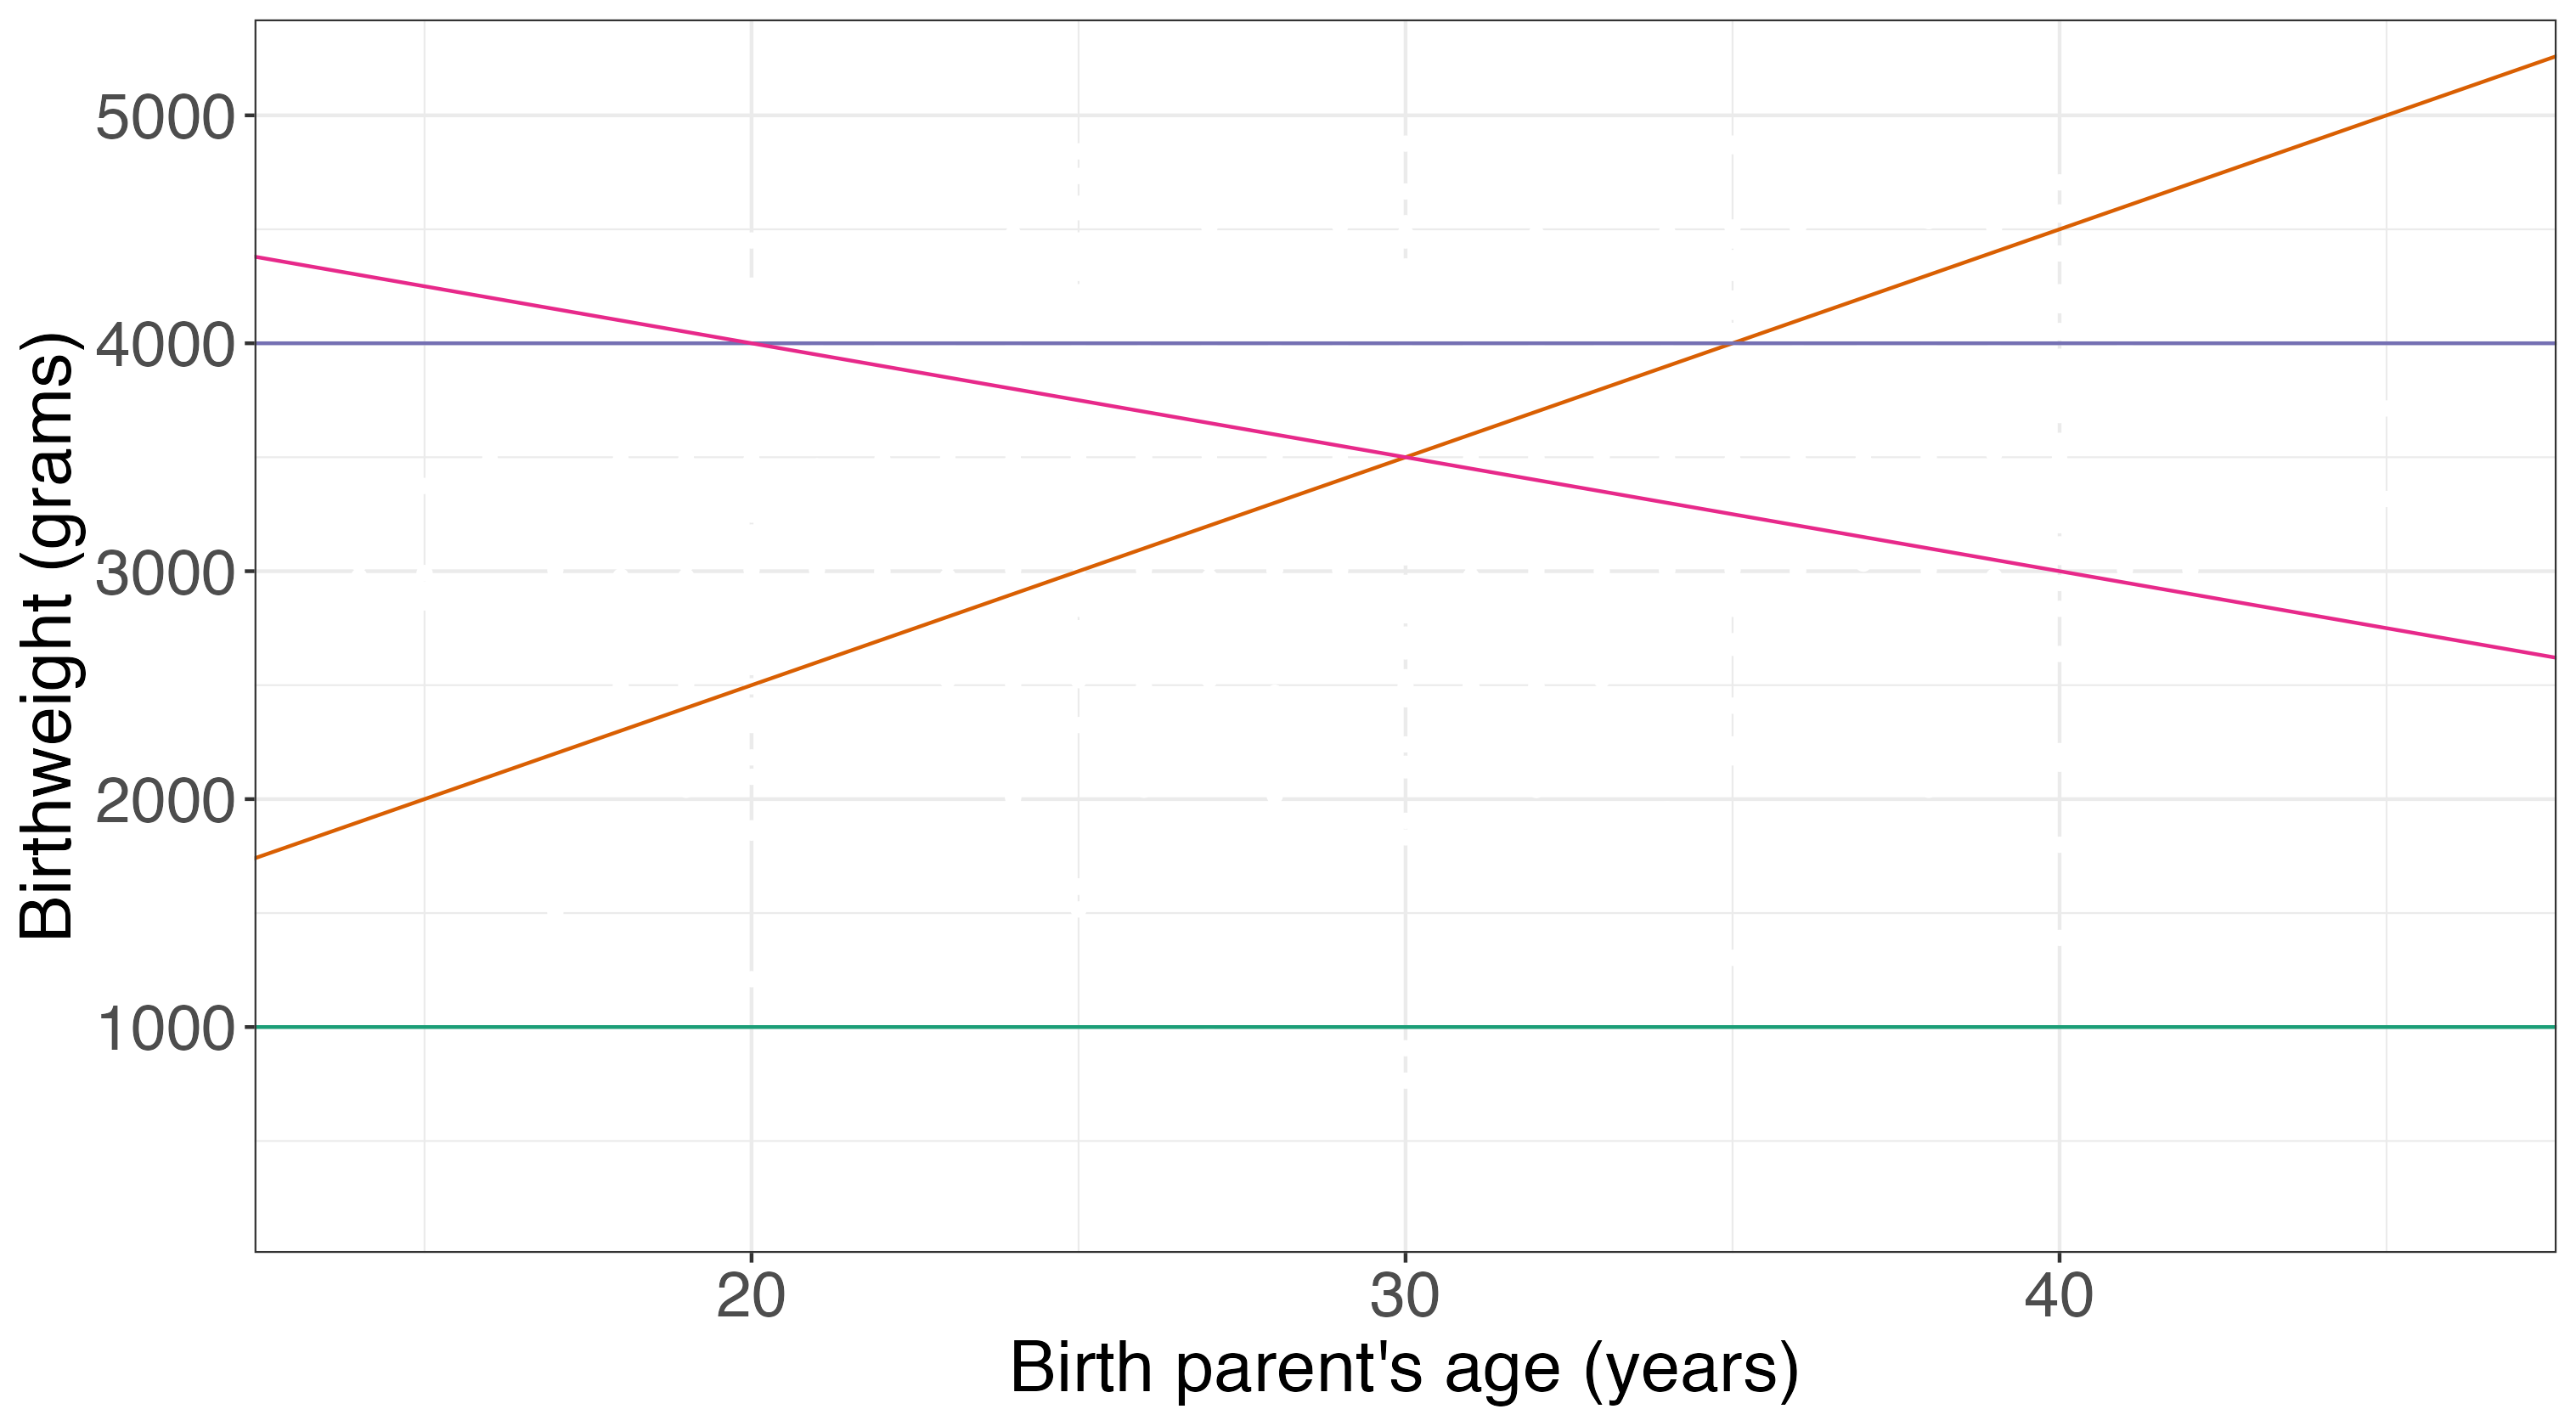
\includegraphics[scale=0.35]{zeroslopes.png}

\end{frame}

\begin{frame}{Why do we care about the slope?}
In which example(s) is there \textbf{no} association between age and birthweight?

\vspace{0.3cm}

\begin{figure}
\centering 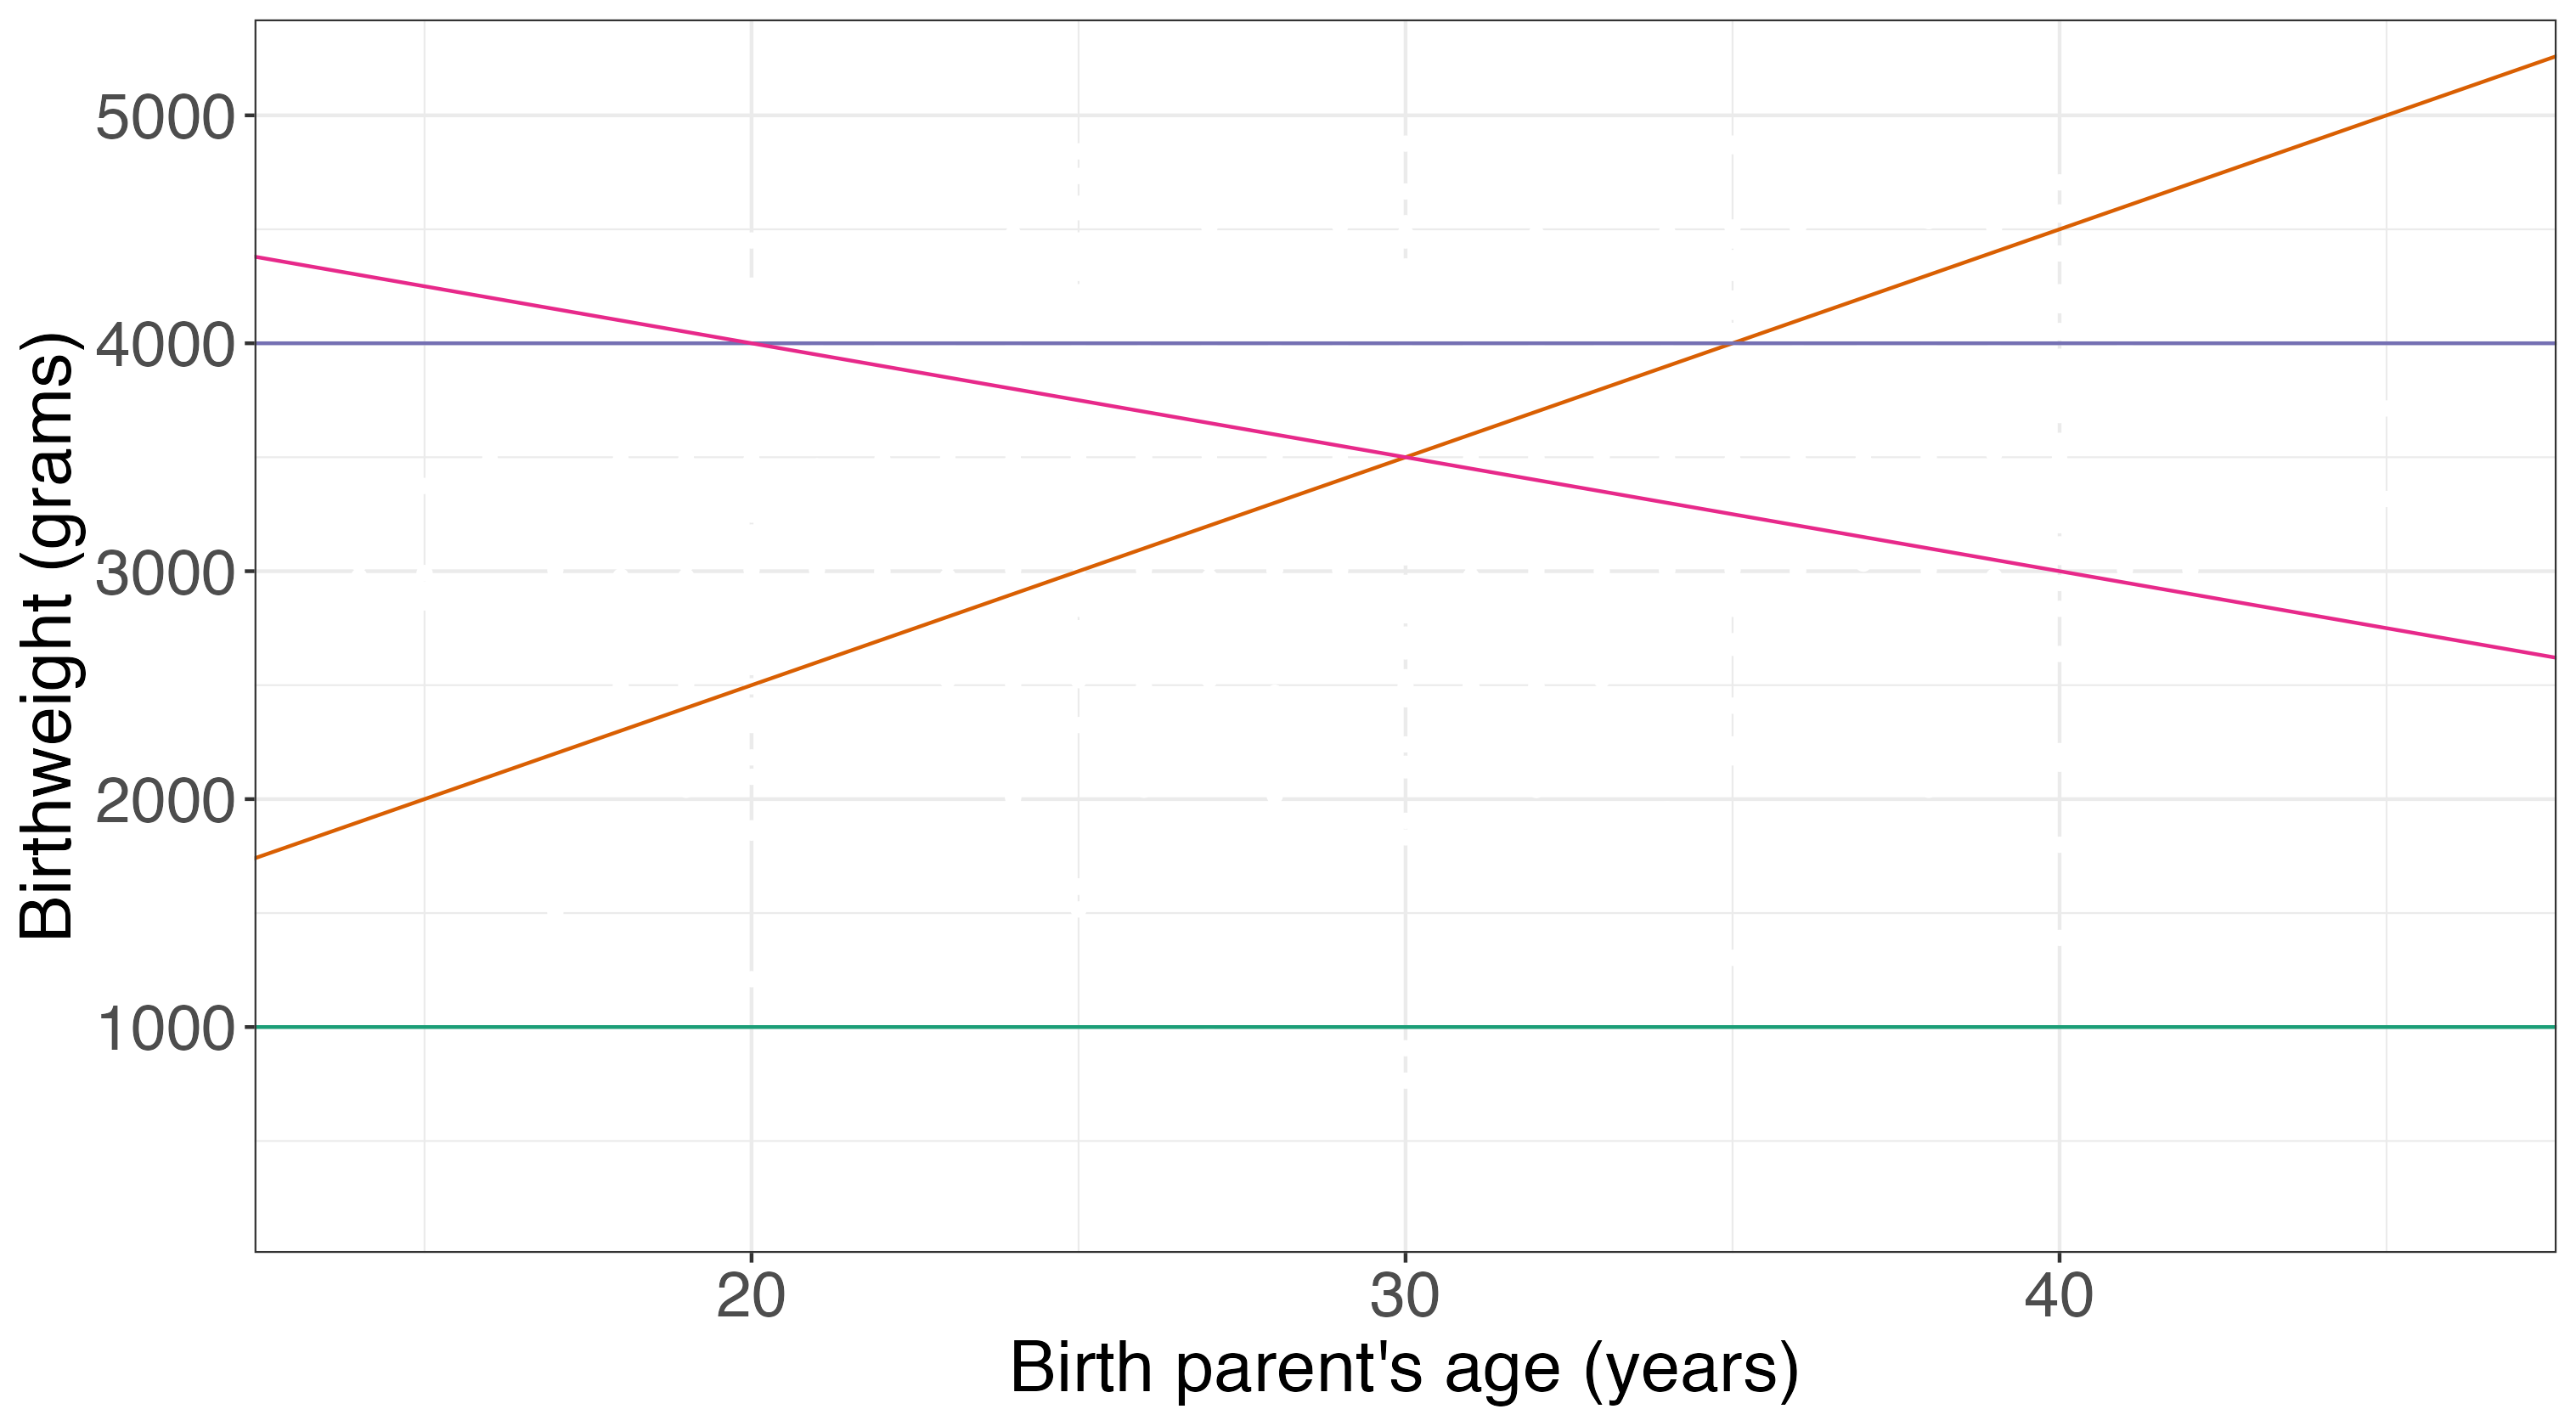
\includegraphics[scale=0.35]{zeroslopes.png}
\end{figure}

\vspace{0.3cm}

\textit{What is the slope in those cases?}

\end{frame}

\begin{frame}{Why do we care about the slope?}
When
\begin{itemize}
	\item $\beta_1 = 0$: there is no linear association between $X$ and $Y$
	\item $\beta_1 > 0$: there is a positive linear association between $X$ and $Y$
	\item $\beta_1 < 0$: there is a negative linear association between $X$ and $Y$
\end{itemize}

\end{frame}

\begin{frame}{Why do we care about the slope?}
When
\begin{itemize}
	\item $\beta_1 = 0$: there is no linear association between $X$ and $Y$
	\item $\beta_1 > 0$: there is a positive linear association between $X$ and $Y$
	\item $\beta_1 < 0$: there is a negative linear association between $X$ and $Y$
\end{itemize}

\vspace{0.3cm}

Consider the \textbf{scientific question:} \textit{is there an association between birth outcomes and age of birth parent?}

\vspace{0.3cm}

We can use linear regression to answer this question:

\begin{enumerate}
	\item Fit the model $E[\text{bwt} \mid \text{age}] = \beta_0 + \beta_1 \times \text{age}$
	\item Check whether or not $\beta_1 = 0$ \textcolor{blue}{(estimate, CI, p-value)}*
\end{enumerate}

\vspace{0.3cm}

* Note: our \textbf{null hypothesis} here (that there is \textit{no} association between birth outcomes and age of birth parent) can be written as $H_0: \beta_1 = 0$

\end{frame}

\begin{frame}{Why do we care about the slope?}
When
\begin{itemize}
	\item $\beta_1 = 0$: there is no linear association between $X$ and $Y$
	\item $\beta_1 > 0$: there is a positive linear association between $X$ and $Y$
	\item $\beta_1 < 0$: there is a negative linear association between $X$ and $Y$
\end{itemize}

\vspace{0.3cm}

Consider the \textbf{scientific question:} \textit{is there an association between birth outcomes and age of birth parent?}

\vspace{0.3cm}

We can use linear regression to answer this question:

\begin{enumerate}
	\item Fit the model $E[\text{bwt} \mid \text{age}] = \beta_0 + \beta_1 \times \text{age}$
	\item Check whether or not $\beta_1 = 0$ \textcolor{blue}{(estimate, CI, p-value)}
\end{enumerate}

\vspace{0.3cm}

What \textbf{statistical question} are we answering? \textit{Is there an association between birthweight and age, where association is quantified by the difference in mean birthweight between age groups}

\end{frame}

\begin{frame}{Hypothesis tests}
Consider the regression model:
$$
E[Y \mid X] = \beta_0 + \beta_1 X
$$
We know that $\beta_1$ quantifies the association between $X$ and $Y$.

\vspace{0.3cm}

To test whether there is a \textit{statistically significant} association between $X$ and $Y$, \textcolor{blue}{we need to test whether $\beta_1 = 0$:}

\begin{itemize}
	\item $H_0: \beta_1 = 0$
	\item $H_1: \beta_1 \neq 0$
\end{itemize}



\end{frame}

\begin{frame}{Hypothesis tests}
Consider the regression model:
$$
E[Y \mid X] = \beta_0 + \beta_1 X
$$
We know that $\beta_1$ quantifies the association between $X$ and $Y$.

\vspace{0.3cm}

To test whether there is a \textit{statistically significant} association between $X$ and $Y$, \textcolor{blue}{we need to test whether $\beta_1 = 0$:}

\begin{itemize}
	\item $H_0: \beta_1 = 0$
	\item $H_1: \beta_1 \neq 0$
\end{itemize}

\vspace{0.3cm}

Interpret the $p$-value as we have before in Chapter 0:
\begin{itemize}
	\item $p < \alpha$: \textbf{reject} $H_0$, ``we have evidence to suggest that $X$ is associated with $Y$"
	\item $p > \alpha$: \textbf{fail to reject} $H_0$, ``we do not have enough evidence to support the hypothesis that $X$ is associated with $Y$"
\end{itemize}

\end{frame}

\subsection{Quantifying uncertainty}

\begin{frame}{Standard errors (SEs) and confidence intervals}
When we estimate regression coefficients, we also want to quantify the \textit{uncertainty} in these estimates. Once we have our standard error, we can calculate a 95\% confidence interval.


\end{frame}

\begin{frame}{Standard errors (SEs) and confidence intervals}

We have two options for 95\% confidence intervals:
\begin{enumerate}
	\item $\hat{\beta} \pm 1.96 \times \hat{SE}(\hat{\beta})$
	\item $\hat{\beta} \pm t_{n-2} \times \hat{SE}(\hat{\beta})$
	\begin{itemize}
		\item If $n = 10$, $t_{n-2} = 2.31$
		\item If $n = 100$, $t_{n-2} = 1.98$
		\item If $n = 1000$, $t_{n-2} = 1.96$
	\end{itemize}
\end{enumerate}

\small (\textit{Recall that the $t$-distribution is defined by it's \textit{degrees of freedom}, which is $n-2$ in the case of simple linear regression with a single predictor})

\vspace{0.3cm}

\normalsize The first option is what we are used to seeing. The latter is what is commonly provided in statistical software. The key takeaway for this course is that \textbf{when n} (our sample size) \textbf{is large}, there is little difference between the confidence intervals from options 1 and 2, and the interpretation of the confidence interval remains the same. If you'd like more details on why statistical software typically provides confidence intervals based on a $t$-distribution, please come ask in office hours!

\end{frame}

\begin{frame}{Interpreting 95\% confidence intervals}
Returning to our example of using linear regression to assess the association between birthweight and birth parent's age, suppose we estimate the slope to be 8.6, with a 95\% confidence interval (4.97, 12.25).

\vspace{0.3cm}

We already interpreted the slope previously:

\vspace{0.3cm}

\textit{Comparing two groups of birth parents who differ by one year in age, the difference in average child's birthweight will be 8.6 grams, with the higher average birthweight in the older of the two groups.}

\vspace{0.3cm}

How would we interpret the confidence interval for this slope estimate? % have them chat with a partner

\end{frame}

\begin{frame}{Interpreting 95\% confidence intervals}
Returning to our example of using linear regression to assess the association between birthweight and birth parent's age, suppose we estimate the slope to be 8.6, with a 95\% confidence interval (4.97, 12.25).

\vspace{0.3cm}

Confidence interval interpretation:

\vspace{0.3cm}

\textit{Comparing two groups of birth parents who differ by one year in age, the difference in average child's birthweight will be 8.6 grams, with the higher average birthweight in the older of the two groups. \textcolor{blue}{Based on a 95\% confidence interval, this estimated difference would not be judged unusual if the true difference were between 4.97 and 12.25 grams.}}

\vspace{0.3cm}

\small Note that this is the same language as the confidence interval interpretation for a mean or difference in means, as in Chapter 0!

\end{frame}

\begin{frame}{Connection between confidence intervals and $p$-values}
\textcolor{blue}{Question:} Suppose we have access to the estimate of the slope (8.6) and a 95\% confidence interval to go with it (4.97, 12.25), as before, where our null hypothesis was that the slope was $0$. What can we say about the $p$-value for this hypothesis test?

\vspace{0.3cm}

\begin{enumerate}
	\item $p < 0.05$
	\item $p = 0.05$
	\item $p > 0.05$
	\item $p < 0.95$
\end{enumerate}

\end{frame}

\begin{frame}{Connection between confidence intervals and $p$-values}
\textcolor{blue}{Question:} Suppose we have access to the estimate of the slope (8.6) and a 95\% confidence interval to go with it (4.97, 12.25), as before, where our null hypothesis was that the slope was $0$. What can we say about the p-value for this hypothesis test?

\vspace{0.3cm}

\begin{enumerate}
	\item \textcolor{blue}{$p < 0.05$}
	\item \sout{$p = 0.05$}
	\item \sout{$p > 0.05$}
	\item \sout{$p < 0.95$}
\end{enumerate}

\vspace{0.3cm}

The 95\% confidence interval does not contain the null hypothesis of $0$, so we reject the null hypothesis. We know that we reject $H_0$ if the p-value is smaller than some pre-specified threshold $\alpha$, which in this case is $1 - 0.95 = 0.05$ since we have a 95\% confidence interval.

\end{frame}


\begin{frame}{Putting it all together \dots}
We've now completed a linear regression ``recipe." After translating a scientific question into a statistical one, the ingredients include:

\vspace{0.3cm}

\begin{itemize}
	\item Determine the \textbf{hypotheses}: $H_0$, $H_1$
	\item Obtain an \textbf{estimate/statistic}: estimated regression coefficient
	\item \textbf{Quantify uncertainty}: 95\% confidence interval for regression coefficient
	\item Perform a \textbf{hypothesis test}: reject, or fail to reject, the null hypothesis based on p-value for regression coefficient
\end{itemize}
\end{frame}

\begin{frame}{Example: birthweight and age}
\begin{enumerate}
	\item \textbf{Scientific question:} is there an \textcolor{orange}{association} between birth outcomes and age of birth parent?
	\item \textbf{Statistical question:} is there a \textcolor{orange}{difference in average} birthweight comparing groups of birth parents that differ in age?
\end{enumerate}
\end{frame}

\begin{frame}{Example: birthweight and age}
\begin{enumerate}
	\item \textbf{Scientific question:} is there an \textcolor{orange}{association} between birth outcomes and age of birth parent?
	\item \textbf{Statistical question:} is there a \textcolor{orange}{difference in average} birthweight comparing groups of birth parents that differ in age?
	\begin{itemize}
		\item \textbf{Population:} all babies born in King County
		\item \textbf{Parameter:} population linear regression slope (diff. in means comparing groups that differ by one year in age)
	\end{itemize}
\end{enumerate}
\end{frame}

\begin{frame}{Example: birthweight and age}
\begin{enumerate}
	\item \textbf{Scientific question:} is there an \textcolor{orange}{association} between birth outcomes and age of birth parent?
	\item \textbf{Statistical question:} is there a \textcolor{orange}{difference in average} birthweight comparing groups of birth parents that differ in age?
	\begin{itemize}
		\item \textbf{Population:} all babies born in King County
		\item \textbf{Parameter:} population linear regression slope (diff. in means comparing groups that differ by one year in age)
	\end{itemize}
	\item Take a \textbf{sample} from the population: 2500 singleton births in King County in 2001, and their birth parents
\end{enumerate}
\end{frame}

\begin{frame}{Example: birthweight and age}
\begin{enumerate}
	\item \textbf{Scientific question:} is there an \textcolor{orange}{association} between birth outcomes and age of birth parent?
	\item \textbf{Statistical question:} is there a \textcolor{orange}{difference in average} birthweight comparing groups of birth parents that differ in age?
	\begin{itemize}
		\item \textbf{Population:} all babies born in King County
		\item \textbf{Parameter:} population linear regression slope (diff. in means comparing groups that differ by one year in age)
	\end{itemize}
	\item Take a \textbf{sample} from the population: 2500 singleton births in King County in 2001, and their birth parents
	\item Perform \textit{statistical inference}:
	\begin{itemize}
		\item Calculate the corresponding \textbf{statistic}: sample linear regression slope (estimated diff. in means comparing groups that differ by one year in age)
	\end{itemize}
\end{enumerate}
\end{frame}

\begin{frame}{Example: birthweight and age}
\begin{enumerate}
	\item \textbf{Scientific question:} is there an \textcolor{orange}{association} between birth outcomes and age of birth parent?
	\item \textbf{Statistical question:} is there a \textcolor{orange}{difference in average} birthweight comparing groups of birth parents that differ in age?
	\begin{itemize}
		\item \textbf{Population:} all babies born in King County
		\item \textbf{Parameter:} population linear regression slope (diff. in means comparing groups that differ by one year in age)
	\end{itemize}
	\item Take a \textbf{sample} from the population: 2500 singleton births in King County in 2001, and their birth parents
	\item Perform \textit{statistical inference}:
	\begin{itemize}
		\item Calculate the corresponding \textbf{statistic}: sample linear regression slope (estimated diff. in means comparing groups that differ by one year in age)
		\item Quantify the uncertainty in your statistic
		\item Perform a hypothesis text
	\end{itemize}
\end{enumerate}
\end{frame}

\begin{frame}{Example: birthweight and age}
\begin{enumerate}
	\item \textbf{Scientific question:} is there an \textcolor{orange}{association} between birth outcomes and age of birth parent?
	\item \textbf{Statistical question:} is there a \textcolor{orange}{difference in average} birthweight comparing groups of birth parents that differ in age?
	\begin{itemize}
		\item \textbf{Population:} all babies born in King County
		\item \textbf{Parameter:} population linear regression slope (diff. in means comparing groups that differ by one year in age)
	\end{itemize}
	\item Take a \textbf{sample} from the population: 2500 singleton births in King County in 2001, and their birth parents
	\item Perform \textit{statistical inference}:
	\begin{itemize}
		\item Calculate the corresponding \textbf{statistic}: sample linear regression slope (estimated diff. in means comparing groups that differ by one year in age)
		\item Quantify the uncertainty in your statistic
		\item Perform a hypothesis text
	\end{itemize}
	\item Make conclusions in context of original question
\end{enumerate}
\end{frame}

\begin{frame}{Example: birthweight and age}
To fit the regression model $E[\text{bwt} \mid \text{age}] = \beta_0 + \beta_1 \times \text{age}$ in \texttt{R} we use the \texttt{lm} function, and the \texttt{confint} function to get confidence intervals (you'll get more practice with this in the HW and discussion section):

\vspace{0.15cm}

\centering 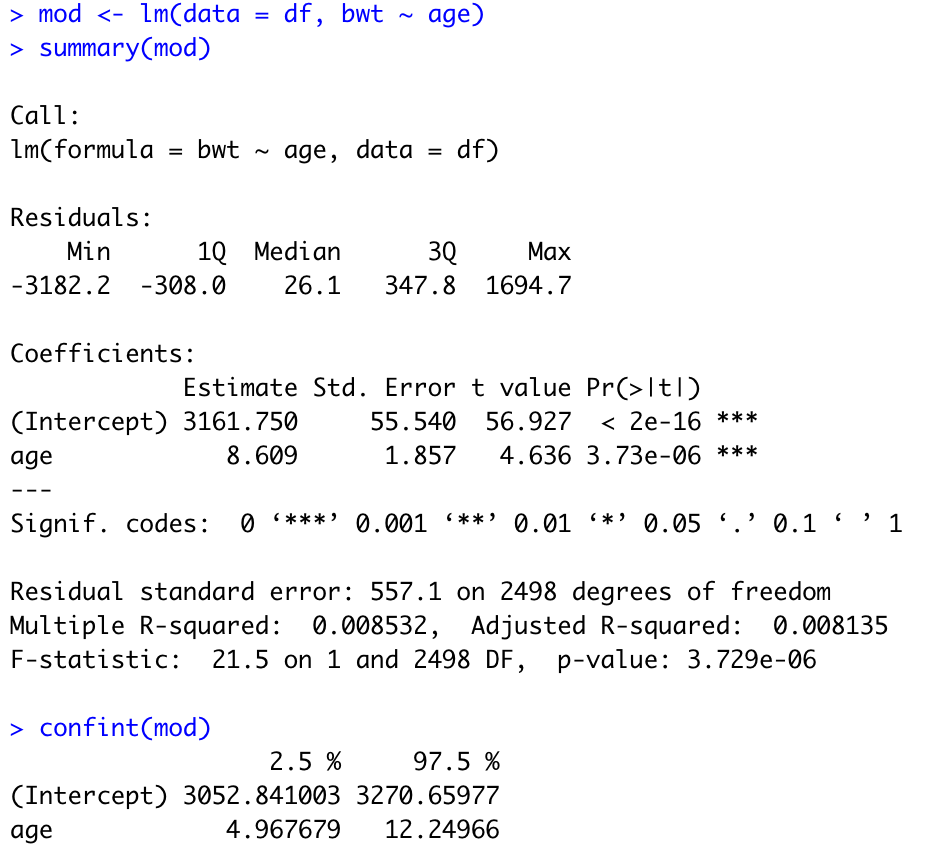
\includegraphics[scale=0.35]{lm_bwt_age.png}

\end{frame}

\begin{frame}{Example: birthweight and age}
The necessary pieces we need to extract from this output are (1) the estimate/statistic, (2) the p-value, and (3) the 95\% confidence interval:

\vspace{0.15cm}

\centering 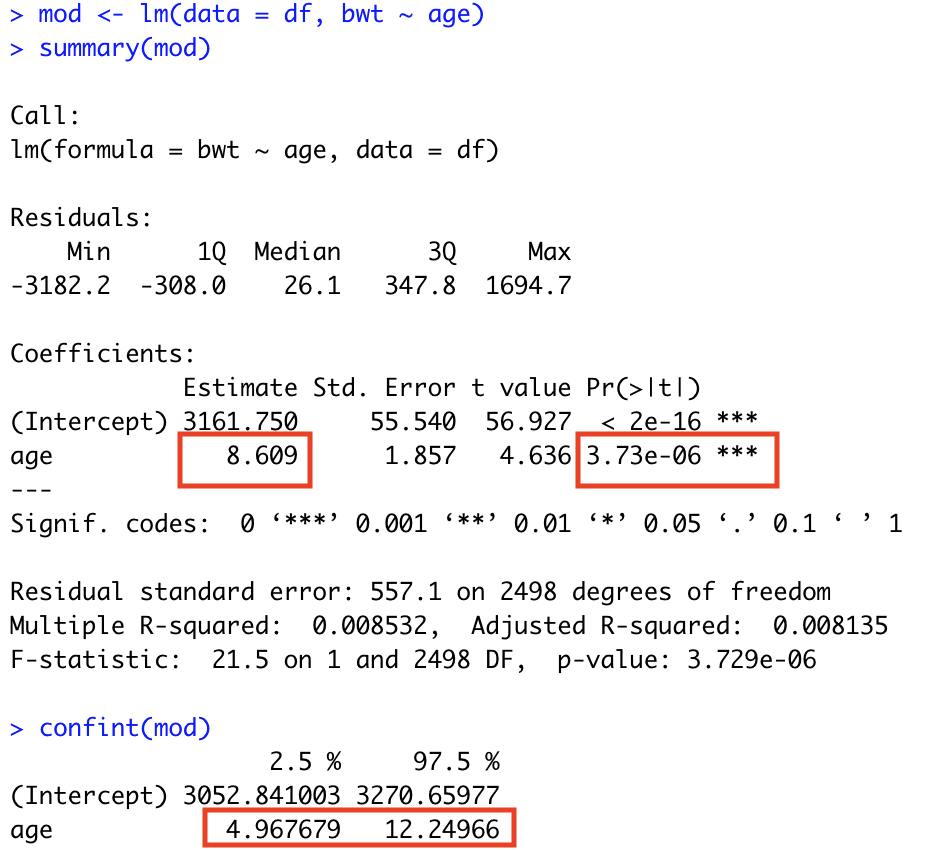
\includegraphics[scale=0.35]{lm_bwt_age2.png}

\end{frame}


\subsection{Assumptions \& diagnostics}

\subsection{Transformations}

\section{Multiple Linear Regression}

\subsection{Adjusting for covariates}

\subsubsection{Confounding (and causal diagrams)}

\subsubsection{Precision variables}

\subsubsection{Effect modification}

\section{Prediction}

\end{document}